\section{Functional and Workflows Description}
% ESO-037611 expects a section called "Functional and Workflows Description" in the DRLD
% "Data Processing Overview" is the term used for the DRLS.
%\section{Data Processing Overview}
\label{sec:data_processing_overview}

The METIS data reduction system runs in different environments and
serves various purposes.  According to the setting, the following
pipeline levels are distinguished~\cite{1618}:

\begin{description}
\item[Quality Control Level 0 (QC0):] The QC0 pipeline runs
  automatically in real time on a dedicated pipeline workstation in
  the instrument control room at the observatory. Its purpose is to
  analyse every FITS file created by the instrument and produce
  quality control parameters that allow assessment of whether the
  observation and instrument performance were within specifications.
  The appropriate reduction recipe is triggered either when a single
  FITS file is delivered to the workstation or when a template is
  finished. The files are classified based on header keywords, grouped
  and associated to the necessary standard calibration files.

\item[Quality Control Level 1 (QC1):] The goal of the QC1 pipeline is
  to produce certified calibration products from calibration
  observations as well as to produce QC parameters that are used to
  check the quality of observations and to monitor observing
  conditions and instrument health.
  The QC1 pipeline is run automatically by ESO in Garching.
  Calibration products and QC parameters are ingested into the ESO Science Archive.

\item[Quality Control Level 2 (QC2):] The QC2 pipeline produces
  Science Data Products compliant with~\cite{ESO-products_standard} as
  well as QC parameters derived from science exposures. It runs
  offline in an automatic way and uses the best calibration products
  for the night of observation (produced by the QC1 pipeline).
  The QC2 pipeline is run automatically by ESO in Garching.
  Science data products and QC parameters are ingested into the ESO Science Archive.

\item[Science-Grade Desktop Environment:] The pipeline recipes are
  delivered to the astronomical community to enable users to reduce
  data in an optimal and interactive way. Recipes can be run from the
  command line using the \lstinline{esorex} front-end or in the
  context of a \lstinline{Reflex}/\ac{EDPS} workflow. While the desktop recipes
  are identical to those used in the QC2 pipeline, the user can change
  recipe parameters to optimise the reduction. Within the
  \lstinline{Reflex}/\ac{EDPS} environment, interactive tools are provided that
  allow the user to assess the quality of individual reduction steps
  and to repeat them with different parameters. The products of this
  pipeline are compliant with~\cite{ESO-products_standard}.

\end{description}


The rest of this document describes the recipes primarily from the perspective of the desktop pipeline.
The QC0, QC1, QC2 pipelines use the subset of these recipes necessary for the goals described above.
Recipes used in the QC0 environment are written such that they can be run in real time, possibly requiring different defaults for processing parameters.


\subsection{Required calibrations}
\label{ssec:calibrations}

Table~\ref{tab:calibrations_per_mode} (taken from
\cite{METIS-calibration_plan}) lists the main calibration steps that
are required for each instrument mode.

%\TODO{Do we apply NCPA + PSF to HCI data? For ADI a simple recipe is foreseen.} The NCPA estimating algorithms are still under study by the HCI team.
%\begin{landscape}
\begin{table}
  \newcommand{\yes}{\tikz\fill[scale=0.35,color=green!50!black](0,.35) -- (.25,0) -- (0.9,.7) -- (.25,.15) -- cycle;}
  \newcommand{\no}{\textcolor{red!50!black}{---}}
    \caption[Overview of required calibrations per instrument mode]{Overview of required calibrations per instrument mode.
    The IFU modes refer to both the nominal configuration and to the extended wavelength configuration. From~\cite{METIS-calibration_plan}.}
  \label{tab:calibrations_per_mode}
  \centering\scriptsize
  \begin{tabularx}{\textwidth}{lXccXccccc}
    \hline
                           & Dark / Linearity & Flat & Wave & Offset type & Telluric & Flux & Distortion & NCPA + PSF & RSRF \\
    \hline\hline
    \CODE{IMG_LM}          & \yes & \yes & \no  & Dither         & \no      & \yes & \yes       & \no        & \no  \\
    \CODE{IMG_LM_(RA/C)VC} & \yes & \yes & \no  & ADI            & \no      & \yes & \yes       & \yes       & \no  \\
 %   \CODE{IMG_LM_CLC}      & \yes & \yes & \no  & ADI            & \no      & \yes & \yes       & \yes       & \no  \\
    \CODE{IMG_LM_APP}      & \yes & \yes & \no  & Dither + ADI   & \no      & \yes & \yes       & \yes       & \no  \\
    \CODE{SPEC_LM}         & \yes & \no  & \yes & Dither along slit & \yes  & \yes & \yes       & \no        & \yes \\
    \CODE{IFU}             & \yes & \no  & \yes & Dither         & \yes     & \yes & \yes       & \no        & \yes \\
    \CODE{IFU_APP}         & \yes & \no  & \yes & Dither\footnote{Dithering for background subtraction + IFU\_APP will not be practical due to AO halo.}  + ADI  & \yes     & \yes & \yes       & \yes       & \yes \\
    \CODE{IFU_(RA/C)VC}    & \yes  & \no  & \yes & ADI            & \yes     & \yes & \yes       & \yes       & \yes \\
   % \CODE{IFU_CLC}         & \yes & \no  & \yes & Dither + ADI   & \yes     & \yes & \yes       & \yes       & \yes \\
    \hline
    \CODE{IMG_N}           & \yes  & \yes & \no  & chop/nod       & \no      & \yes & \yes       & \no        & \no  \\
    \CODE{IMG_N_CVC}       & \yes  & \yes & \no  & three-point chopping & \no & \yes & \no       & \yes       & \no  \\
 %   \CODE{IMG_N_CLC}       & \no  & \yes & \no  & out-of-field chopping & \no & \yes & \no      & \yes       & \no  \\
    \CODE{SPEC_N_LOW}      & \yes  & \no  & \yes & chop/nod along slit & \yes & \yes & \yes      & \no        & \yes \\
    \hline
  \end{tabularx}
\end{table}
%\end{landscape}
\FloatBarrier

%%%
\subsection{Imaging in LM and N}
\label{ssec:overview_lm_imaging}

% HB 20230731: This note is not really necessary I think.
%\textbf{Note: The pipeline layout has been modified compared to the
%  PDR design in order to achieve better modularity. Basic reduction
%  and background subtraction have been split into two recipes that now
%  are applied to both standard calibration and science data. ADI recipes have been added since PDR however integration of \ac{HCI}
%  into this workflow requires more work: \ac{HCI} images will be treated
%  the same way at least through basic reduction, possibly through
%  background subtraction. \ac{ADI} combination may require a separate
%  recipe, at least for some \ac{HCI} configurations.}

The purpose of the pipeline is to correct or remove contributions from
the instrument, telescope, and atmosphere and produce science-grade
data products.  In the case of the METIS imaging modes the main
contributions to correct or remove are dark current, flatfield, bad
pixels, and, most importantly, thermal background emission from the
sky and the telescope. Further effects include persistence,
cross-talk, geometric distortions, etc. The final product of the
imaging pipeline is one or more image(s) that are flux-calibrated in units of
photons/s/pixel against a standard star.
Several images can be stacked into a single possibly mosaiced image.

Due to the differences in characteristics between the HAWAII2RG
detector used for imaging in the L and M bands and the GeoSnap
detector used for the N band, the operational concept for the two
imager subsystems are quite different. This induces differences in the
way the data have to be reduced.

The GeoSnap detector has more stable gain than AQUARIUS detector,
which was still in the baseline at PDR\@.  Chopping is still necessary, albeit
at a lower frequency of a few Hz, and a chop/nod technique, which meets the
specific ELT requirements (Section~\ref{sssec:nbandsbackgroundsubtracion}),
will be employed  for background subtraction.  As the dark
signal is automatically removed when the exposures from the different
chop and nod positions are combined no master dark is required for the
reduction of science data. The GeoSnap data is also flat fielded.

Observations and reduction of LM band data with the HAWAII2RG detector
can proceed as in the near infrared. After dark subtraction and
flat-fielding, the background is estimated from a series of dithered
science exposures or from exposures on a nearby blank patch of sky.

The association maps for the current designs of the imaging pipelines
in~LM and~N are shown in Figs.~\ref{fig:IMG_LM_Assomap}
and~\ref{fig:IMG_N_Assomap}, respectively.

%\TODO{For \ac{HCI} data, \ac{ADI} may need to be part of reduction recipe if
%  individual background subtracted images are the goal?} We provide ADI recipes since PDR.

\begin{landscape}
  \begin{figure}
    \centering
    \resizebox{\linewidth}{!}{%% IMG_LM_assomap_tikz.tex
%% Created by Oliver Czoske
%%
%% 2019-02-26: Changed to LM only
%% 2019-02-26: Try to align it with the recipe flow
%% 2020-09-07: Pipeline redesign

\sffamily


% ADDING NEW DEFINITIONS -------------------------------------------- start
\definecolor{listingbg}{gray}{0.95}
\definecolor{darkgreen}{rgb}{0.0, 0.7, 0.0}
\definecolor{darkblue} {rgb}{0.0, 0.0, 0.7}
\definecolor{cyan} {rgb}{0.0, 0.4, 0.4}
\definecolor{darkred}  {rgb}{0.7, 0.0, 0.0}
\definecolor{darkorange}{rgb}{1.0, 0.49, 0.0}
\definecolor{violett}{rgb}{255, 0, 255}
\definecolor{turq}{rgb}{0.0, 0.7, 0.8}
\definecolor{fits}{rgb}{0.4, 0.1, 1}


\makeatletter
\lstdefinestyle{RAWstyle}{%
  basicstyle=\ttfamily\color{black}%
  \lst@ifdisplaystyle\scriptsize\fi}

\lstdefinestyle{PARstyle}{%
  basicstyle=\ttfamily\color{black}%
  \lst@ifdisplaystyle\scriptsize\fi}

\lstdefinestyle{DRLstyle}{%
  basicstyle=\ttfamily\color{black}%
  \lst@ifdisplaystyle\scriptsize\fi}

\lstdefinestyle{RECstyle}{%
  basicstyle=\ttfamily\color{black}%
  \lst@ifdisplaystyle\scriptsize\fi}

\lstdefinestyle{QCstyle}{%
  basicstyle=\ttfamily\color{black}%
  \lst@ifdisplaystyle\scriptsize\fi}

\lstdefinestyle{TPLstyle}{%
  basicstyle=\ttfamily\color{black}%
  \lst@ifdisplaystyle\scriptsize\fi}

\lstdefinestyle{PRODstyle}{%
  basicstyle=\ttfamily\color{black}%
  \lst@ifdisplaystyle\scriptsize\fi}

\lstdefinestyle{EXTCALIBstyle}{%
  basicstyle=\ttfamily\color{black}%
  \lst@ifdisplaystyle\scriptsize\fi}

\lstdefinestyle{STATCALIBstyle}{%
  basicstyle=\ttfamily\color{black}%
  \lst@ifdisplaystyle\scriptsize\fi}
\makeatother

%%% This file contains definitions of shapes and nodes used
%%% for a recipe workflow
%%% Author       : Oliver Czoske
%%% Created      : 2021-03-03
%%% Last Changed : 2021-03-03
%%% Changes:
%%%

\usetikzlibrary{
  shapes.misc,
  positioning,
  calc,
  arrows.meta}

%% All connecting lines have an arrow
\tikzset{
  connection_arrow/.style={->, >=Latex[open], thick}
}

%% Start and stop buttons (black disks, stop with ring)
%% These are pics, use as
%%         \pic (name) [above of=..] {picname};
\tikzset{
  start/.pic = {
    \node (-m) at (0, 0){};
    \filldraw [fill=black] (0, 0) circle (0.2);
  }
}

\tikzset{
  stop/.pic = {
    \node (-m) at (0, 0){};
    \node (-t) at (0, -0.3){};
    \filldraw [fill=black] (0, 0) circle(0.2);
    \draw[black] (0, 0) circle (0.3);
  }
}


%%%% Various boxes and their colours
%%%% These are nodes, use as
%%%% \node (name) [type, location]  {text};

\definecolor{stepcolor}{RGB}{210,169,188}
\definecolor{rawcolor}{RGB}{205,205,205}
\definecolor{externalcolor}{RGB}{183,255,255}
\definecolor{calibcolor}{RGB}{255,250,216}
\definecolor{calproductcolor}{RGB}{185,184,237}
\definecolor{qcproductcolor}{RGB}{255,201,165}
\definecolor{sciproductcolor}{RGB}{197,219,183}
\definecolor{framecolor}{RGB}{127,13,65}

\tikzset{
  %% template : the template(s) that trigger(s) the recipe
  template/.style={
    rectangle,
    draw=black,
    minimum width=4.0cm,
    minimum height=0.5cm,
    align=center
  },
  %% input : the input files
  input/.style={
    rectangle,
    fill=rawcolor,
    minimum width=4.0cm,
    minimum height=0.75cm,
%     text width=3cm,
    align=center
  },
  %% calib : calibration input
  calib/.style={
    rectangle,
    fill=calibcolor,
    minimum width=4.0cm,
    minimum height=0.75cm,
%     text width=3cm,
    align=center
  },
  %% external : external input
  external/.style={
    rectangle,
    fill=externalcolor,
    minimum width=4.0cm,
    minimum height=0.75cm,
%     text width=3.5cm,
    align=center
  },
  %% params : parameters
  params/.style={
    rectangle,
    draw=red,
    thick,
    minimum width=4.0cm,
    minimum height=0.75cm,
%     text width=3cm,
    align=center
  },
  %% redstep : a reduction step
  %%      ("step" is predefined and can't be used)
  redstep/.style={
    rectangle,
    rounded corners=0.2cm,
    fill=stepcolor,   %%% define colour!
    minimum width=4.0cm,
    minimum height=1cm,
%     text width=3cm,
    align=center
  },
  %% connection : connection to input or output
  connection/.style={
    circle,
    fill=black,
    minimum size=0.15cm,
    inner sep=0pt
  },
  %% sciproduct : a science product
  sciproduct/.style={
    rectangle,
    fill=sciproductcolor,
    minimum width=4.0cm,
    minimum height=0.75cm,
%     text width=3.5cm,
    align=center
  },
  %% calproduct : a calibration product
  calproduct/.style={
    rectangle,
    fill=calproductcolor,
    minimum width=4.0cm,
    minimum height=0.75cm,
%     text width=3.5cm,
    align=center
  },
  %% frame : frame around the recipe
  %% This is a path, use as
  %%    \draw [frame] (upper left) rectangle (lower right);
  frame/.style={framecolor, very thick, dashed}
}


%%% Picture: flow chart
\begin{tikzpicture}[on grid=false,node distance=0.8cm]

  \matrix (recipes) [column sep=0.1cm, row sep=1cm]{
    % The matrix has colums
    % detlin_*, dark_*, flat_*, std_*, sci1_*, sci2_*, adi
    %
    % The matrix has rows
    % *_raw, *_dark, *_flat, *_std, *_sci1, *_sci2, *_prod

    % Row *_raw
    \node [above] (lin_raw){%
      \recipebox{DETLIN}{det\_lingain}
    };
    &
    \node [above] (pers_raw){%
        \recipebox{PERSISTENCE}{persistence\_map}
    };
    &
    \node [above] (dist_raw){%
      \recipebox{DISTORTION}{lm\_img\_distortion}
    };
    &
    \node[above] (dark_raw) {%
      \recipebox{DARK}{det\_dark}
    };
    &
    \node[above] (flat_raw){%
      \recipebox{FLAT}{lm\_img\_flat}
    };
    &
    \node[above] (all1_raw){%
      \recipebox{SCIENCE, STD}{lm\_img\_basic}
    };
    &
    \node[above] (all2_raw){%
      \recipebox{SCIENCE, STD}{lm\_img\_background}
    };
    &
    \node[above] (std_raw){%
      \recipebox{PHOT STD}{lm\_img\_std\_process}
    };
    &
    \node[above] (sci1_raw){%
      \recipebox{SCIENCE}{lm\_img\_sci\_calibrate}
    };
    &
    \node[above] (sci2_raw){%
      \recipebox{SCIENCE}{lm\_img\_sci\_coadd}
    };

   % \node[above] (sci2_raw){%     % needs width parameter to box
   %  \begin{tcolorbox}[%
   %    width=4.5cm,
   %    colback=recipecolor]
   %    \centering lm\_img\_sci\_postprocess
   %  \end{tcolorbox}};
   %&
   %\node[above] (adi_raw){%
   %  \recipenotitlebox{adi\_postprocess}
   %};
   \\

    %%% Calibration products
    % Row *_lin
    \node (lin_lin) [statcalfile]{\hyperref[dataitem:linearity_2rg]{\STATCALIB{LINEARITY_2RG}}}; &
    \node (pers_lin)[empty]{}; &
    \node (dist_lin)[empty]{}; &
    \node (dark_lin)[empty]{}; &
    \node (flat_lin)[connection]{}; &
    \node (all1_lin)[connection]{}; &
    \node (all2_lin)[empty]{}; &
    \node (std_lin)[empty]{}; &
    \node (sci1_lin)[empty]{}; &
    \node (sci2_lin)[empty]{}; \\

    % Row persistence
    \node (lin_pers)[empty]{}; &
    \node (pers_pers)[extcalfile]{\STATCALIB{PERSISTENCE_MAP}}; &
    \node (dist_pers)[empty]{}; &
    \node (dark_pers)[empty]{}; &
    \node (flat_pers)[connection]{}; &
    \node (all1_pers)[connection]{}; &
    \node (all2_pers)[empty]{}; &
    \node (std_pers)[empty]{}; &
    \node (sci1_pers)[empty]{}; &
    \node (sci2_pers)[empty]{}; \\

    % Row *_dark
    \node (lin_dark) [empty]{}; &
    \node (pers_dark) [empty]{}; &
    \node (dist_dark) [empty]{}; &
    \node (dark_dark) [calibproduct]{\hyperref[dataitem:master_dark_2rg]{\PROD{MASTER_DARK_2RG}}}; &
    \node (flat_dark)[connection]{}; &
    \node (all1_dark)[connection]{}; &
    \node (all2_dark)[empty]{}; &
    \node (std_dark)[empty]{}; &
    \node (sci1_dark)[empty]{}; &
    \node (sci2_dark) [empty]{}; \\

    % Row *_flat
    \node (lin_flat) [empty]{}; &
    \node (pers_flat) [empty]{}; &
    \node (dist_flat)[empty]{}; &
    \node (dark_flat)[empty]{}; &
    \node (flat_flat) [calibproduct]{\hyperref[dataitem:master_flat_2rg]{\PROD{MASTER_FLAT_2RG}}}; &
    \node (all1_flat)[connection]{}; &
    \node (all2_flat)[empty]{}; &
    \node (std_flat)[empty]{}; &
    \node (sci1_flat)[empty]{}; &
    \node (sci2_flat) [empty]{}; \\

    % Row *_all1
    \node (lin_all1)[empty]{}; &
    \node (pers_all1) [empty]{}; &
    \node (dist_all1)[empty]{}; &
    \node (dark_all1)[empty]{}; &
    \node (flat_all1)[empty]{}; &
    \node (all1_all1)[calibproduct]{\hyperref[dataitem:std_reduced]{\PROD{STD_REDUCED}}}; &
    \node (all2_all1)[calibproduct]{\hyperref[dataitem:std_bkg_sub]{\PROD{STD_BKG_SUB}}}; &
    \node (std_all1)[connection]{}; &
    \node (sci1_all1)[empty]{}; &
    \node (sci2_all1) [empty]{}; \\

% Row *_all2
    \node (lin_all2) [empty]{}; &
    \node (pers_all2) [empty]{}; &
    \node (dist_all2)[empty]{}; &
    \node (dark_all2)[empty]{}; &
    \node (flat_all2)[empty]{}; &
    \node (all1_all2)[scienceproduct]{\hyperref[dataitem:sci_reduced]{\PROD{SCI_REDUCED}}}; &
    \node (all2_all2)[scienceproduct]{\hyperref[dataitem:sci_bkg_sub]{\PROD{SCI_BKG_SUB}}}; &
    \node (std_all2)[empty]{}; &
    \node (sci1_all2)[connection]{}; &
    \node (sci2_all2) [empty]{}; \\

    % Row *_dist
    \node (lin_dist) [empty]{}; &
    \node (pers_dist) [empty]{}; &
    \node (dist_dist)[statcalfile]{\hyperref[dataitem:distortion_tab]{\STATCALIB{DISTORTION_TAB}}}; &
    \node (dark_dist)[empty]{}; &
    \node (flat_dist) [empty]{}; &
    \node (all1_dist)[empty]{}; &
    \node (all2_dist)[empty]{}; &
    \node (std_dist)[empty]{}; &
    \node (sci1_dist)[connection]{}; &
    \node (sci2_dist) [empty]{}; \\

    % Row *_std
    \node (lin_std) [empty]{}; &
    \node (pers_std) [empty]{}; &
    \node (dist_std)[empty]{}; &
    \node (dark_std)[extcalfile]{\hyperref[dataitem:fluxstd_catalog]{\EXTCALIB{FLUXSTD_CATALOG}}}; &
    \node (flat_std)[empty]{}; &
    \node (all1_std)[empty]{}; &
    \node (all2_std)[empty]{}; &
    \node (std_std)[connection]{}; &
    \node (sci1_std)[empty]{}; &
    \node (sci2_std) [empty]{}; \\

    % Row *_sci1
    \node (lin_sci1) [empty]{}; &
    \node (pers_sci1) [empty]{}; &
    \node (dist_sci1)[empty]{}; &
    \node (dark_sci1)[empty]{}; &
    \node (flat_sci1)[empty]{}; &
    \node (all1_sci1)[empty]{}; &
    \node (all2_sci1)[empty]{}; &
    \node (std_sci1)[calibproduct]{\hyperref[dataitem:fluxcal_tab]{\PROD{FLUXCAL_TAB}}}; &
    \node (sci1_sci1)[connection]{}; &
    \node (sci2_sci1)[empty]{}; \\

    % Row *_sci2
    \node (lin_sci2) [empty]{}; &
    \node (pers_sci2) [empty]{}; &
    \node (dist_sci2)[empty]{}; &
    \node (dark_sci2)[empty]{}; &
    \node (flat_sci2)[empty]{}; &
    \node (all1_sci2)[empty]{}; &
    \node (all2_sci2)[empty]{}; &
    \node (std_sci2)[empty]{}; &
    \node (sci1_sci2) [scienceproduct]{\hyperref[dataitem:lm_sci_calibrated]{\PROD{LM_SCI_CALIBRATED}}}; &
    \node (sci2_sci2) [connection]{}; \\

    % Row *_prod
    \node(lin_prod) [empty]{}; &
    \node(pers_prod) [empty]{}; &
    \node(dist_prod) [empty]{}; &
    \node(dark_prod) [empty]{}; &
    \node(flat_prod) [empty]{}; &
    \node(all1_prod) [empty]{}; &
    \node(all2_prod) [empty]{}; &
    \node(std_prod) [empty]{}; &
    \node(sci1_prod) [empty]{}; &
    \node (sci2_prod)[scienceproduct]{\hyperref[dataitem:lm_sci_coadd]{\PROD{LM_SCI_COADD}}}; \\
  };    % end matrix

  \node (t1) at ($(dist_raw)!0.5!(dark_raw)$){};
  \node (t2) at ($(dist_prod)!0.5!(dark_prod)$){} ;
  \draw [thick,dashed] ([yshift=8mm]t1.north) -- ([yshift=-8mm]t2.south);



  %% Vertical connections
  \draw [arrow] (lin_raw)  -- (lin_lin);
  \draw [arrow] (pers_raw) -- (pers_pers);
  \draw [arrow] (dist_raw) -- (dist_dist);
  \draw [arrow] (dark_raw) -- (dark_dark);
  \draw [arrow] (flat_raw) -- (flat_flat);
  \draw [arrow] (all1_raw) -- (all1_all1);
  \draw [arrow] (all1_all1) -- (all1_all2);
  \draw [arrow] (std_all1) -- (std_sci1);
  \draw [arrow] (sci1_all2) -- (sci1_sci2);
  \draw [arrow] (sci2_sci2) -- (sci2_prod);
%  \draw [arrow] (adi_sci2) -- (adi_prod);

  %% Horizontal connections
  \draw [match] (lin_lin)   -- (all1_lin);
  \draw [match] (pers_pers) -- (all1_pers);
  \draw [match] (dark_dark) -- (all1_dark);
  \draw [match] (flat_flat) -- (all1_flat);
  \draw [match] (all1_all1) -- (all2_all1);
  \draw [match] (all2_all1) -- (std_all1);
  \draw [match] (all1_all2) -- (all2_all2);
  \draw [match] (all2_all2) -- (sci1_all2);
  \draw [match] (sci1_std) -- (sci1_sci1);
  \draw [match] (dist_dist) -- (sci1_dist);
  \draw [match] (dark_std) -- (std_std);
  \draw [match] (std_sci1) -- (sci1_sci1);
  \draw [match] (sci1_sci2) -- (sci2_sci2);

  %% Legend
  \matrix (legend) [draw, fill=gray!15, above right, row sep=0.3cm,
    column 1/.style={anchor=base},
    column 2/.style={anchor=base west}]
    at ([yshift=0ex]current bounding box.south west){%
      \node (leg_recipe) [recipe] {lm\_img\_flat};
      & \node {recipe}; \\
      \node (leg_calproduct) [calibproduct] {MASTER\_DARK\_2RG};
      & \node {calib.\ product}; \\
      \node (leg_sciproduct)[scienceproduct] {LM\_SCI\_REDUCED};
      & \node {science product}; \\
      \node (leg_statcalfile)[statcalfile] {MASTER\_RSRF};
      & \node {static calib.\ file};\\
      \node (leg_calfile)[extcalfile]{FLUXSTD\_CATALOG};
      & \node {external calib.\ file}; \\

    \draw [arrow,fill=black] (0,0.4) -- (0,-0.3);  %% should be centred relative to column
    & \node {processing step}; \\

    \draw (-1, 0.5ex) -- (1,0.5ex) node [connection,yshift=0cm]{};
    & \node {product match}; \\
  };    %% end matrix (legend)

\end{tikzpicture}
}
    \caption[Reduction cascade and association map for imaging in L and
      M]{Association map for imaging in the LM band. The figure shows only
      the primary product created from each recipe; for a full list of
      products refer to the recipe descriptions in
      Sect.~\ref{ssec:recipes_img_lm}. The dashed line separates
      calibration tasks that are done at AIT or infrequently during
      operations (left) from daily tasks (right). The prefix ``\texttt{metis\_}'' has been
      omitted from the recipe names to improve clarity.}
    \label{fig:IMG_LM_Assomap}
  \end{figure}
\end{landscape}

\begin{landscape}
\begin{figure}
  \centering
    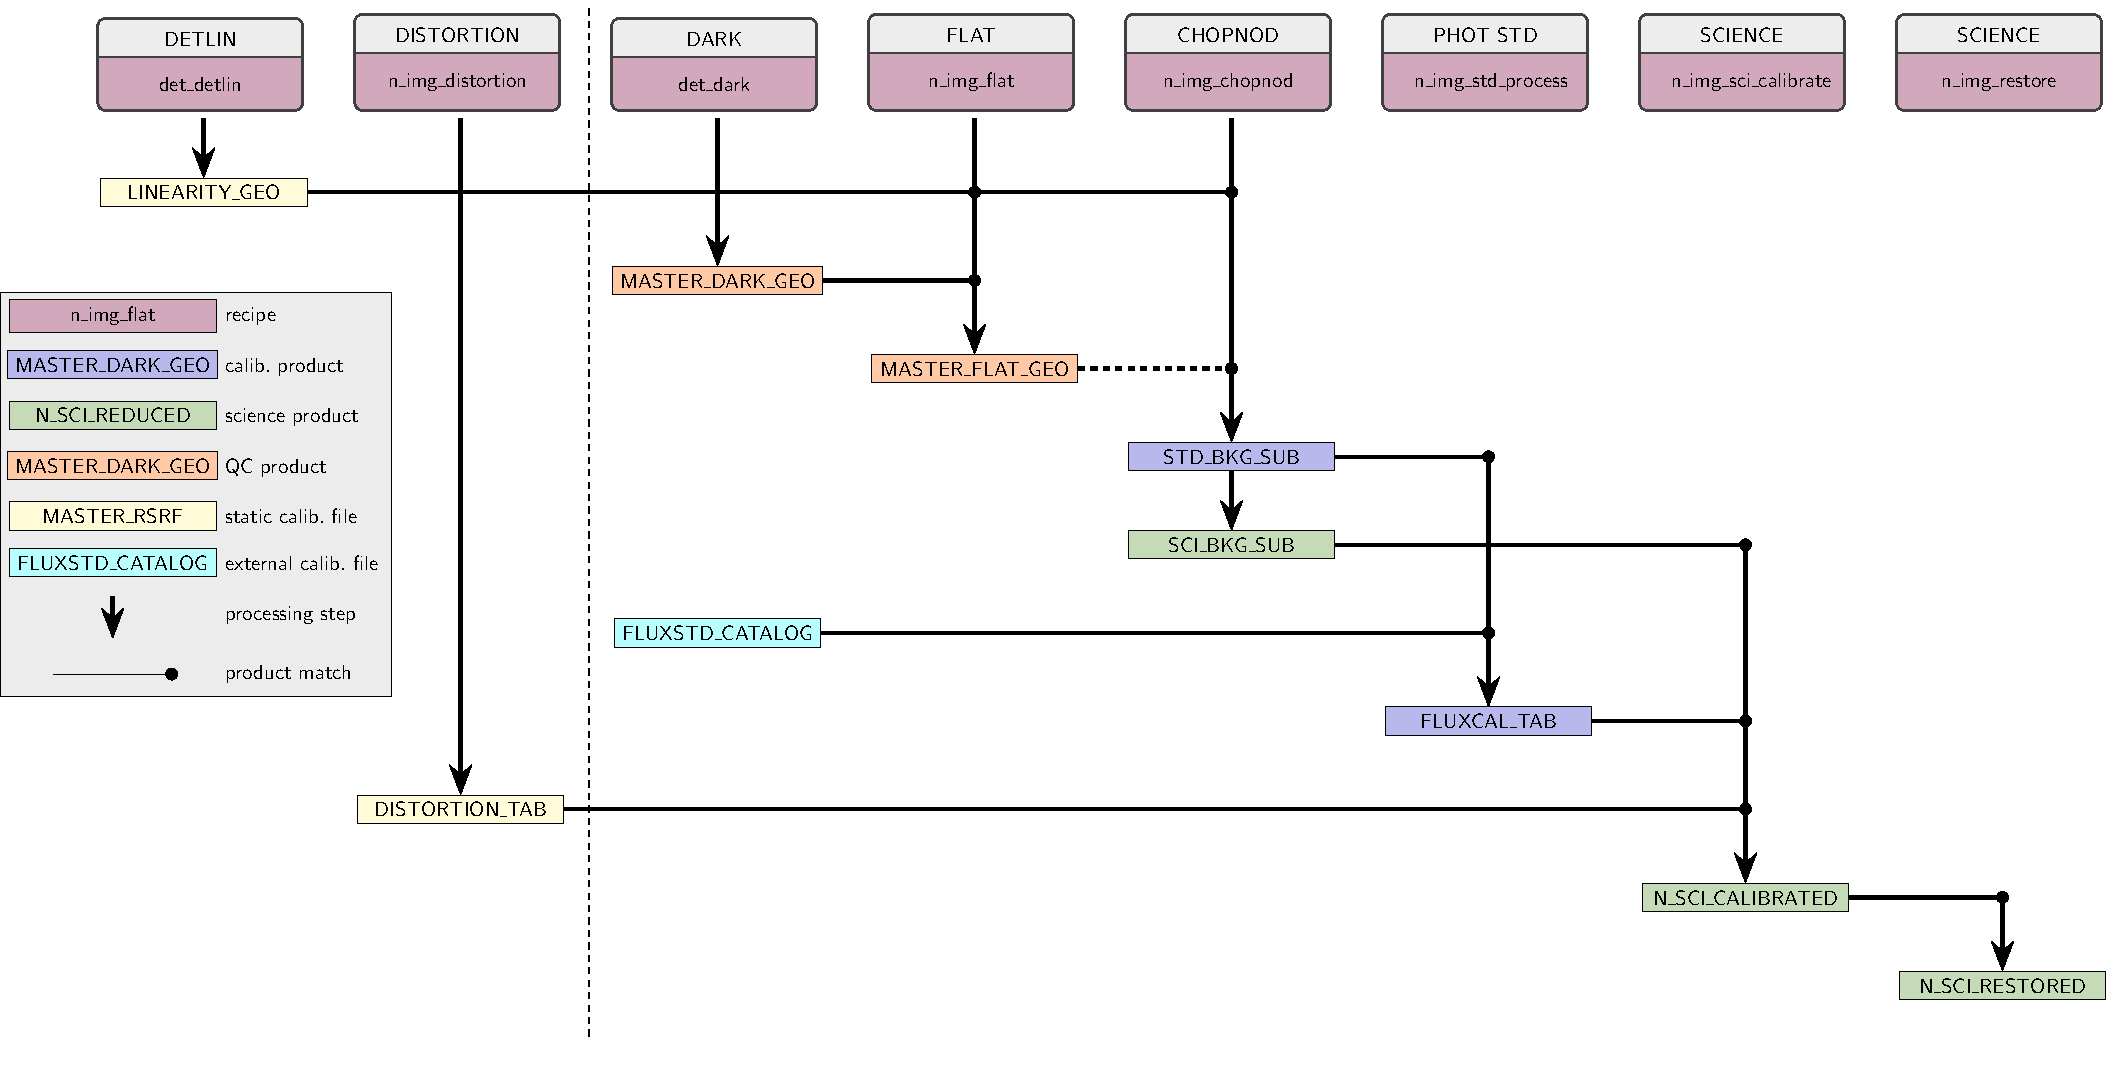
\includegraphics{IMG_N_assomap_tikz}
    \caption[Reduction cascade and association map for imaging in N]{%
      Association map for imaging in the N band. The figure shows
      only the primary product created from each recipe; for a full
      list of products refer to the recipe descriptions in
      Sect.~\ref{ssec:recipes_img_n}. The dashed line separates
      calibration tasks that are done at AIT or infrequently during
      operations (left) from daily tasks (right). The prefix ``\texttt{metis\_}'' has
      been omitted from the recipe names to improve clarity.}
    \label{fig:IMG_N_Assomap}
  \end{figure}
\end{landscape}

%%%%%%%%%%%%%%%%%%%%%%%%%%%%%%%%%%%%%%%%%%%%%%%%%%%%%%
%%% Local Variables:
%%% TeX-master: "METIS_DRLD"
%%% End:


%%%
\subsection{Long-Slit Spectroscopy in L/M- and N-bands}\label{lss:overview}
\subsubsection{The workflow cascades}\label{lss:cascade_overview}
The purpose of the pipeline is to correct or remove contributions from
the instrument, telescope, and atmosphere and generate science-grade
data products for the L/M- and N-band \ac{LSS}
mode. Since the detector properties are not fully specified, especially of the new Geosnap, we currently assume
basically the same reduction cascade for both spectral ranges LM and
N, respectively. The only major difference at the time being is the absence of \ac{WCU} laser sources in the N-band, which are only available during \ac{AIT} phase to generate a first guess of the pixel-to-wavelength relation. Therefore the first guess wavelength solution in the N-band will be based on that \ac{AIT} data. As we assume the instrument to be very stable, that approach should be sufficient for the low-resolution N-band spectroscopy. In the LM range, two fix-frequency lasers ($@3.39$µm and $@5.26$µm) and one tuneable ($4.68....4.78$µm) is foreseen in the \ac{WCU} to be taken on daily basis (cf. \cite{METIS-calibration_plan}). Although mainly foreseen to be used for the high-resolution spectroscopy \ac{LMS} mode, we can use these laser sources for the LM-band \ac{LSS} as well.

Special emphasis has to be drawn to the effects of the Earth's
atmosphere in several respects:
\begin{itemize}
\item Wavelength calibration: Absorption/emission features are intended to be
  used for the wavelength calibration. Thus, a good knowledge on /
  identification of these features is crucial for the accuracy of the
  wavelength calibration.
\item Telluric correction: In the MIR regime telluric absorption is
  one of the most dominant effects visible in spectra. Modelling
  approaches like \texttt{molecfit} heavily rely on accurate
  atmospheric input profiles, which represent the actual state and
  composition of the Earth's atmosphere. This especially applies to
  the \ac{PWV} content since this is the most
  dominant and most variable species.
\item Atmospheric dispersion: \ac{METIS} will have \ac{ADC}s compensating the
  effect of atmospheric dispersion. However, for technical reasons
  these ADCs are fixed at several positions. This means that the
  compensation is only partially. This leads to two practical effects:
  (a) wavelength-dependent slit losses, and (b) distortions in both,
  the spatial and the spectral direction (see \cite{METIS-ADC_study}
  for more details). For both, the pipeline needs to correct
  for. It is foreseen to determine these slitlosses on yearly basis with a separate calibration task (cf. \cite{METIS-calibration_plan}) and create a slit-loss table to be included in the static calibration database.
\end{itemize}

%However, to keep flexibility and independence of both branches, we
%define different recipes for the time being, although they will be
%mostly based on the same algorithms. We therefore focus here on the LM-band only.

Figures~\ref{Fig:LMLssAssomap1} and \ref{Fig:LMLssAssomap2} show the reduction cascade and the association map for the recipes handling L/M-long-slit
spectroscopy data.  Table~\ref{Tab:LMLssDatProc} contains the data processing table for this mode. For the N-band \ac{LSS} mode the cascade and the data processing table is given in Fig.\ref{Fig:NLssAssomap} and Table~\ref{Tab:NLssDatProc}, respectively (cf. also Fig.~\ref{Fig:LSScascadelegend}).

In general, there are four major steps in each of the two cascades:
\begin{itemize}
    \item \textbf{Preparation step:} This contains the recipes, which are invoked only rarely, e.g. after major instrument interventions, or on monthly/yearly basis to update the static calibration database. These recipes are therefore not shown in the cascade in Figs.~\ref{Fig:LMLssAssomap1}/\ref{Fig:LMLssAssomap2} and \ref{Fig:NLssAssomap} and the corresponding data processing tables. In case of the \ac{LSS} pipeline this concerns the creation of the gain maps/linearity checks (see Section~\ref{sssec:metis_det_lingain}), the determination of the slit losses induced by the fixed positions of the ADCs (cf. Section~\ref{sssec:adc_slitlosses} and Section "Calibration of slit losses" in Calibration plan \cite{METIS-calibration_plan}) and the zero position of the chopping mirror (see Section~\ref{ssec:metisimgchophome} and Section "Chopper Home Position" in \cite{METIS-calibration_plan} for more details). T
    \item \textbf{Basic steps}: The basic steps aim for correcting the detector influence, in particular the dark correction and the determination of the master \ac{RSRF}.
    \item \textbf{Calibration/correction steps}: This is the main part which incorporates the order trace detection, distortion, wavelength and flux correction.
    \item \textbf{Post-calibration steps}: After havig calibrated spectra at hand, the last step is the telluric absorption correction.
\end{itemize}

\begin{figure}[ht]
  \centering
  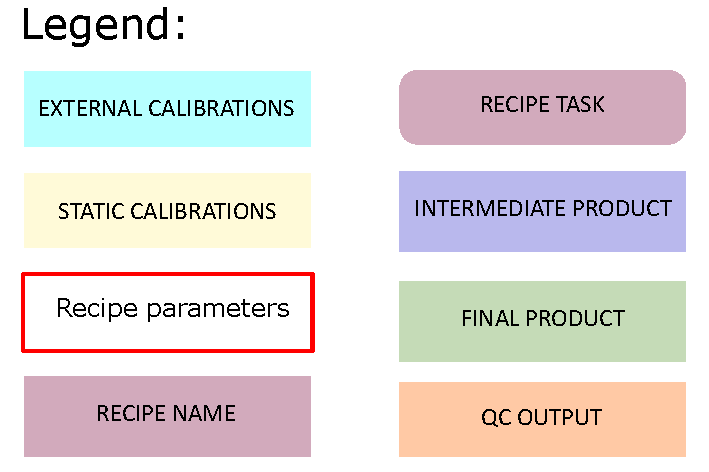
\includegraphics[width=0.4\textheight]{figures/legend.pdf}
  \caption[Legend]{Legend of the coloured boxes in the \ac{LSS} cascades.}
  \label{Fig:LSScascadelegend}
\end{figure}
\clearpage

\begin{sidewaysfigure}[ht]
  \centering
  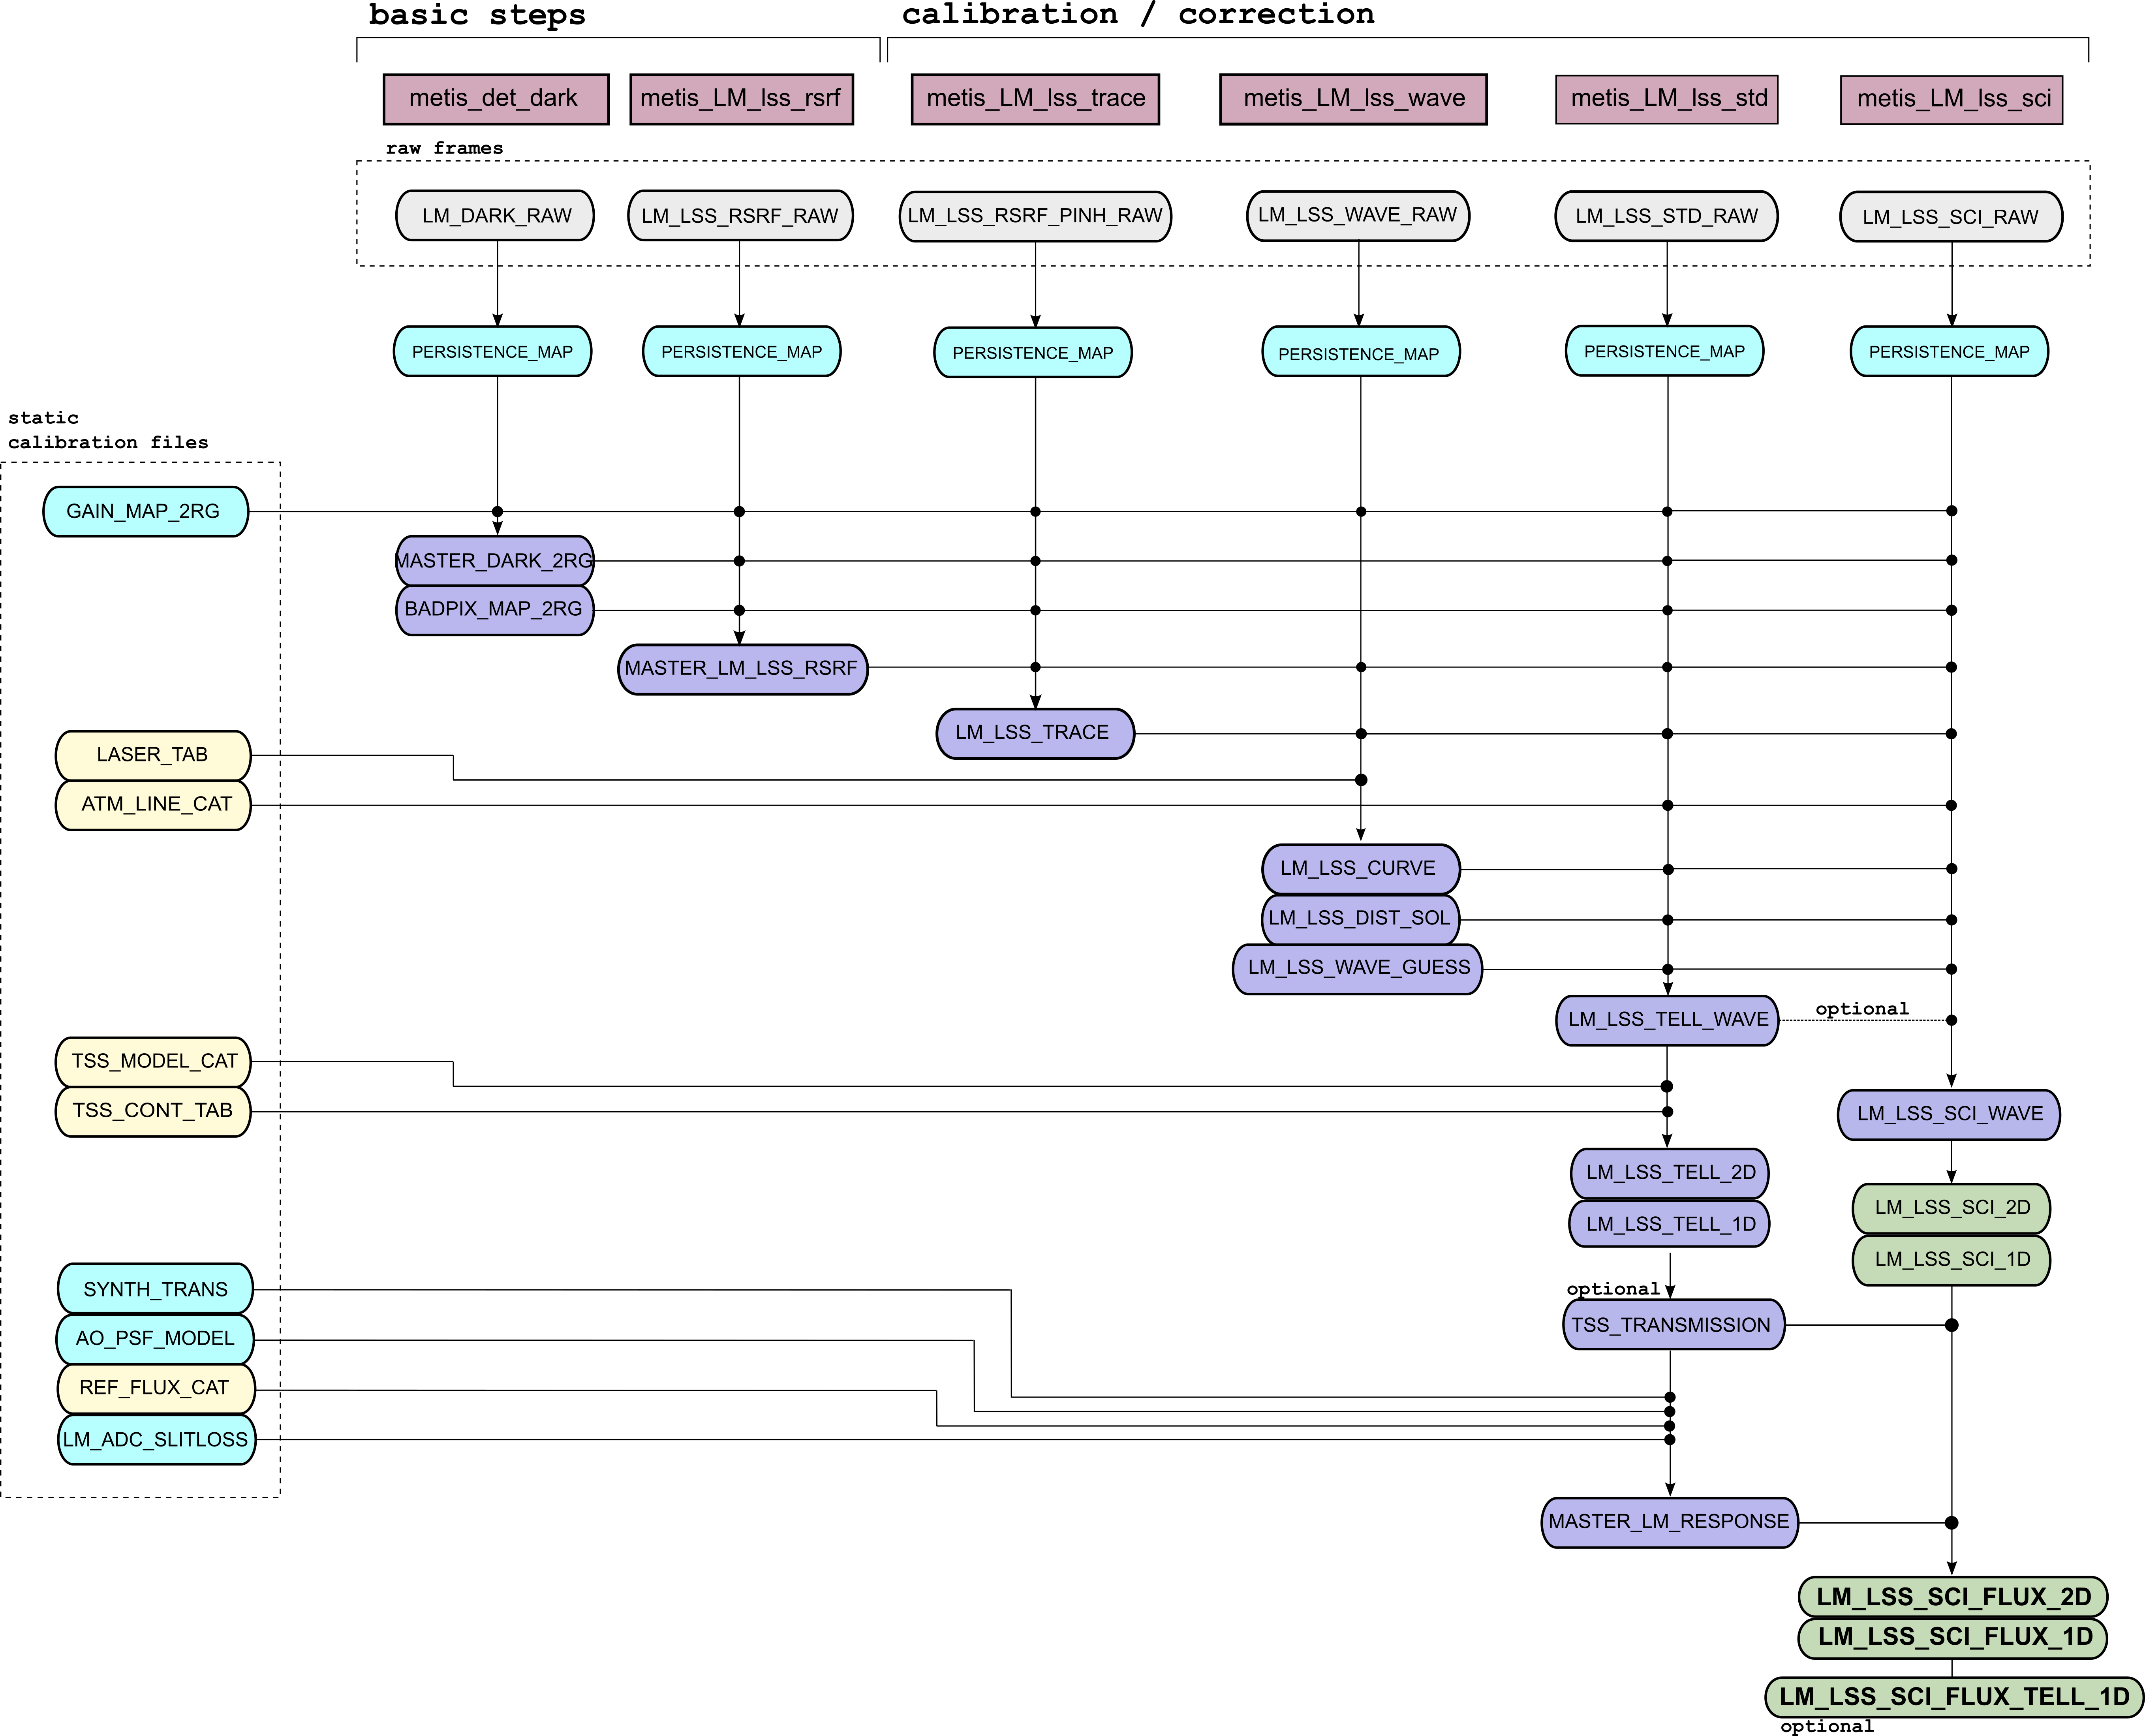
\includegraphics[width=0.9\textheight]{figures/LM_LSS_pipeline_wf_draft_latest_part_1_v0.80.png}
  \caption[Reduction cascade and association map for LM long-slit
  spectroscopy]{Part 1 of the reduction cascade and association map for long-slit
    spectroscopy in the LM bands.  }
  \label{Fig:LMLssAssomap1}
\end{sidewaysfigure}

\begin{sidewaysfigure}[ht]
  \centering
  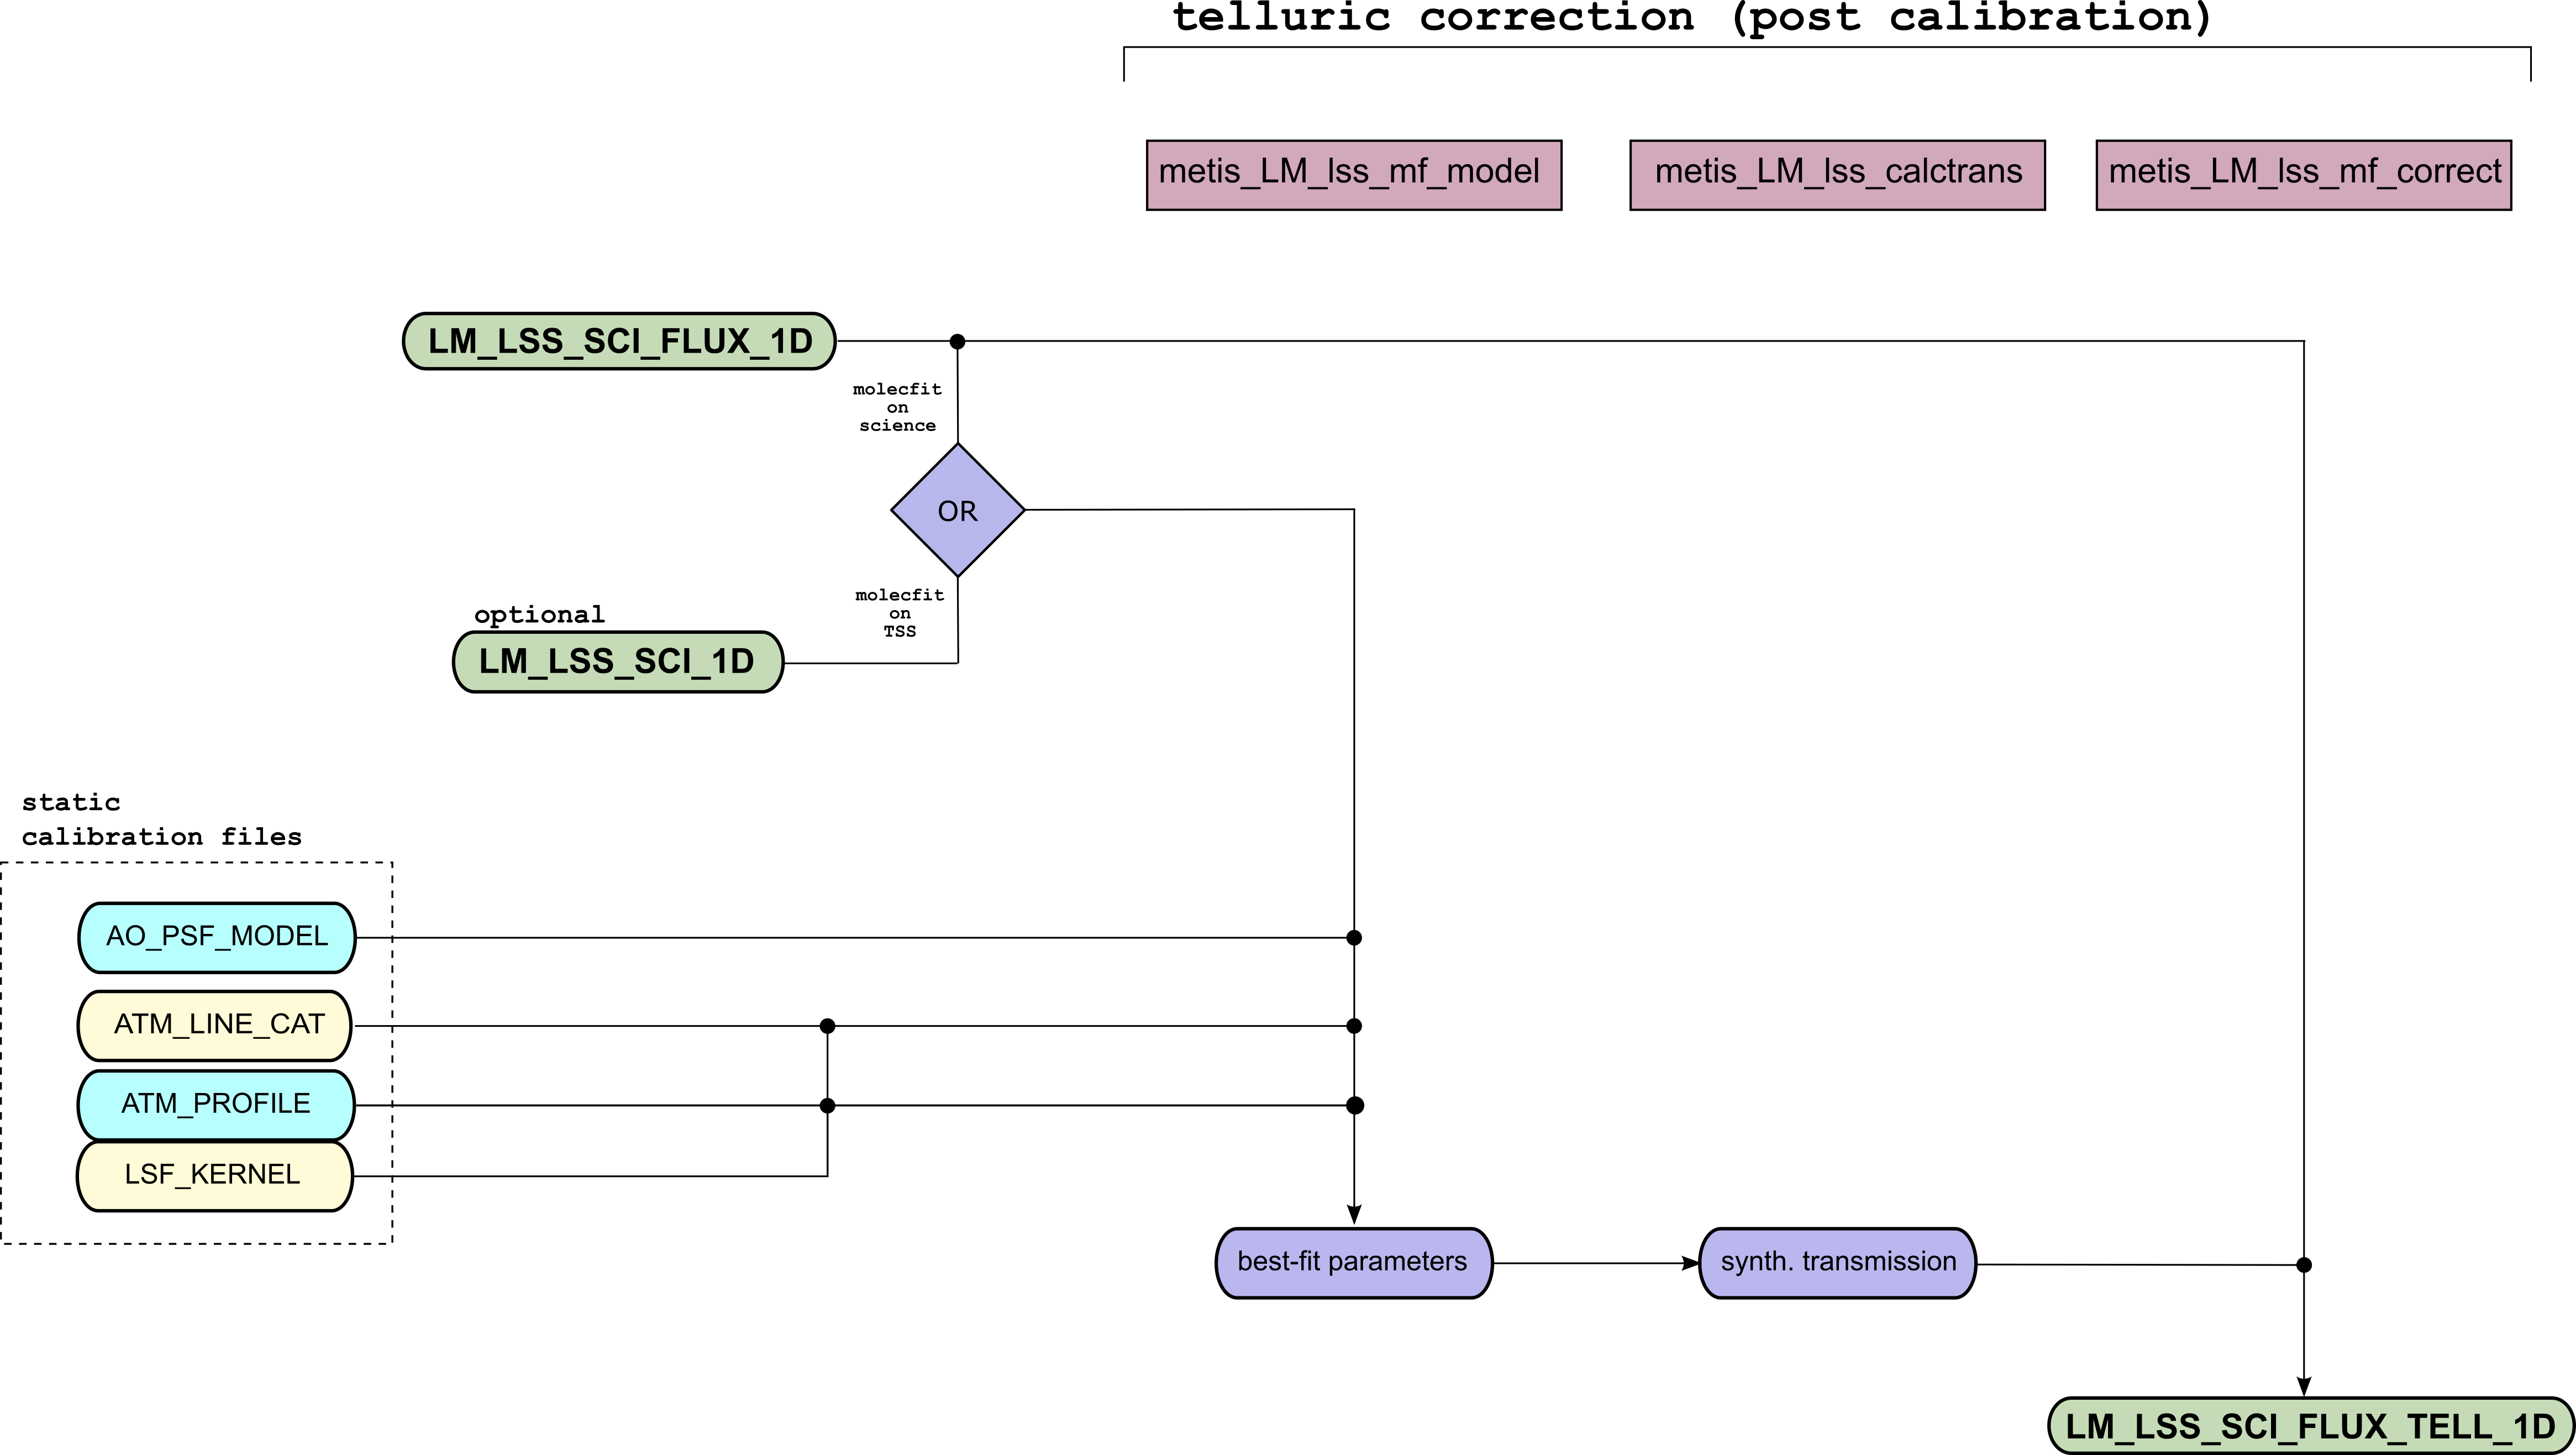
\includegraphics[width=0.8\textheight]{figures/LM_LSS_pipeline_wf_draft_latest_part_2_v0.80.png}
  \caption[Reduction cascade and association map for LM long-slit
  spectroscopy]{Part 2 of the reduction cascade and association map for long-slit
    spectroscopy in the LM bands.  }
  \label{Fig:LMLssAssomap2}
\end{sidewaysfigure}


% \begin{sidewaysfigure}[ht]
%   \centering
%   \includegraphics[width=0.9\textheight]{figures/NQ_LSS_pipeline_wf_draft_latest.png}
%   \caption[Reduction cascade and association map for N long-slit
%   spectroscopy]{Reduction cascade and association map for long-slit
%     spectroscopy in the N band.  }
%   \label{Fig:NQLssAssomap}
% \end{sidewaysfigure}


%% ---- Table: LM long-slit spectroscopy
\begin{sidewaystable}
  \footnotesize
  \begin{center}
    \caption[Data Processing table for LM long-slit spectroscopy]{%
      Data Processing table for LM long-slit spectroscopy
      calibration mode; }\bigskip
    \label{Tab:LMLssDatProc}
    \begin{tabular}{|l|l|l|l|l|l|}
      \hline
      Data Type   & Classification & Recipe (Level)	& FITS Keywords & static CalibDB & Products\\
    (Templates) & Keywords	 & Processing steps	&		&	  &	\\
    \hline
    \TPL{DARK}	& \CODE{DPR.CATG==CALIB} & \hyperref[sssec:metis_det_dark]{\REC{metis_det_dark}} & Exposure time	&	\hyperref[dataitem:gainmap2rg]{\PROD{GAIN_MAP_2RG}}& Averaged dark frame\\
    		& \CODE{DPR.TYPE==DARK}  &			&		&	& Bad pixel map\\
    		& \CODE{DPR.TECH==IMAGE}  &			&		&	& \\
    \hline
    \TPL{FLAT}	& \CODE{DPR.CATG==CALIB} & \hyperref[rec:lsslmrsrf]{\REC{metis_LM_lss_rsrf}} & Exposure time	& \hyperref[dataitem:gainmap2rg]{\PROD{GAIN_MAP_2RG}}	& Averaged, normalized flatfield\\
    		& \CODE{DPR.TYPE==FLAT}  &			&	Grism	& 	& \\
    		& \CODE{DPR.TECH==SPECTRUM}  &			&	Slit	&	& \\
    \hline
         	& \CODE{DPR.CATG==CALIB} &\hyperref[rec:lsslmtrace]{\REC{metis_LM_lss_trace}} & Exposure time	& \hyperref[dataitem:gainmap2rg]{\PROD{GAIN_MAP_2RG}}	& Order location\\
    		& \CODE{DPR.TYPE==FLAT}  &			&		&	& (polynomial fit)\\
    		& \CODE{DPR.TECH==SPECTRUM}  &			&		&	& \\
    \hline
    \TPL{WAVE,LASER} & \CODE{DPR.CATG==CATG} &\hyperref[rec:lsslmwave]{\REC{metis_LM_lss_wave}} & Exposure time &  \hyperref[dataitem:gainmap2rg]{\PROD{GAIN_MAP_2RG}} & wavelength solution\\
    		& \CODE{DPR.TYPE==WAVE,LASER}   &			   & Grism & \hyperref[dataitem:lasertab]{\STATCALIB{LASER_TAB}} &\\
    		& \CODE{DPR.TECH==SPECTRUM}  &			& Slit		&	& \\
    		& \CODE{PRO.CATG==SPECTRUM}   &  &  & & \\
    \hline
    \TPL{FLUX,STD} & \CODE{DPR.CATG==CALIB} & \hyperref[rec:lsslmstd]{\REC{metis_LM_lss_flux}}& Object name (Flux STD) & \hyperref[dataitem:gainmap2rg]{\PROD{GAIN_MAP_2RG}} & Instrumental\\
    		& \CODE{DPR.TYPE==FLUX,STD}   &			   & Exposure time & \hyperref[dataitem:atmlinecat]{\EXTCALIB{ATM_LINE_CAT}} & response function\\
    		& \CODE{DPR.TECH==SPECTRUM}  &			&	Grism	&	\hyperref[dataitem:lmsynthtrans]{\STATCALIB{LM_SYNTH_TRANS}}& \\
    		& \CODE{PRO.CATG==SPECTRUM}   &  & Slit & \hyperref[dataitem:lmadcslitloss]{\STATCALIB{LM_ADC_SLITLOSS}} & \\
    		& & & & \hyperref[dataitem:aopsfmodel]{\EXTCALIB{AO_PSF_MODEL}} &\\    
    		& & & & \hyperref[dataitem:reffluxcat]{\STATCALIB{REF_FLUX_CAT}} &\\    \hline
    \TPL{SCIENCE} & \CODE{DPR.CATG==SCIENCE} & \hyperref[rec:lsslmsci]{\REC{metis_LM_lss_sci}} & Object name &  \hyperref[dataitem:gainmap2rg]{\PROD{GAIN_MAP_2RG}} & Science grade spectrum\\
    		& \CODE{DPR.TYPE==OBJECT}   &			   & Exposure time & \hyperref[dataitem:lmadcslitloss]{\STATCALIB{LM_ADC_SLITLOSS}} &\\
    		& \CODE{DPR.TECH==SPECTRUM}  &			&	Grism	& \hyperref[dataitem:atmlinecat]{\EXTCALIB{ATM_LINE_CAT}}	& \\
    		& \CODE{PRO.CATG==SPECTRUM}   &  & Slit  &  & \\
    \hline
            & \CODE{DPR.CATG==SCIENCE} & \hyperref[rec:LMLSSmfmodel]{\REC{metis_LM_lss_mf_model}} & Object name & \hyperref[dataitem:lsfkernel]{\STATCALIB{LSF_KERNEL}}	 & Best-fit \\
    		& \CODE{DPR.TYPE==OBJECT}   &			  & & \hyperref[dataitem:atmprofile]{\EXTCALIB{ATM_PROFILE}}  & \texttt{molecfit} parameters\\
    		& \CODE{DPR.TECH==TBD}  &			&		& \hyperref[dataitem:atmlinecat]{\EXTCALIB{ATM_LINE_CAT}}	& \\
    		& \CODE{PRO.CATG==TBD}   &  &  & start parameter set & \\
    \hline
            & \CODE{DPR.CATG==SCIENCE} &  \hyperref[rec:LMLSSmfcalctrans]{\REC{metis_LM_lss_mf_calctrans}} & Object name & \hyperref[dataitem:atmlinecat]{\EXTCALIB{ATM_LINE_CAT}}	 & synthetic \\
    		& \CODE{DPR.TYPE==LSS}   &		&	   &   & Transmission curve\\
    		& \CODE{DPR.TECH==TBD}  &			&		& 	& \\
    		& \CODE{PRO.CATG==TBD}   &  &  & & \\
    \hline
            & \CODE{DPR.CATG==SCIENCE} &  \hyperref[rec:LMLSSmfcorrect]{\REC{metis_LM_lss_mf_correct}} & Object name & 	 & Absorption corrected\\
    		& \CODE{DPR.TYPE==LSS}   &			   & & synthetic Transmission curve  & science spectrum\\
    		& \CODE{DPR.TECH==TBD}  &			&		&	& \\
    		& \CODE{PRO.CATG==TBD}   &  &  & & \\
    \hline
    \end{tabular}
  \end{center}
\end{sidewaystable}

\begin{sidewaysfigure}[ht]
  \centering
  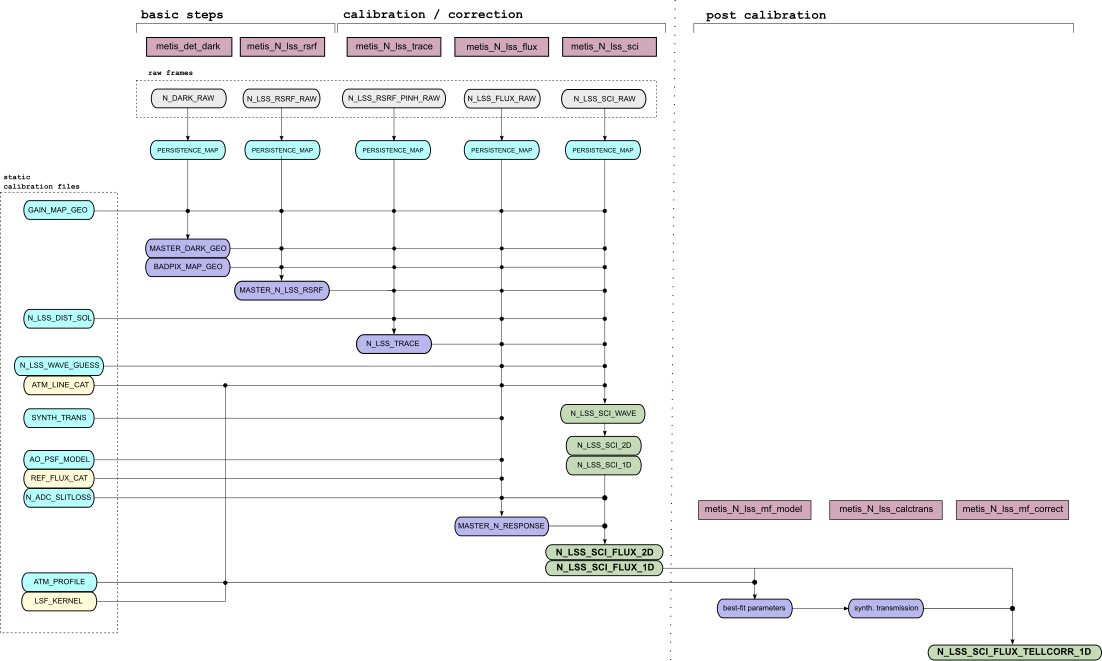
\includegraphics[width=0.9\textheight]{figures/N_LSS_pipeline_wf_draft_latest_v0.74.png}
  \caption[Reduction cascade and association map for N long-slit
  spectroscopy]{Reduction cascade and association map for long-slit
    spectroscopy in the N bands. }
  \label{Fig:NLssAssomap}
\end{sidewaysfigure}

%% ---- Table: N long-slit spectroscopy
\begin{sidewaystable}
  \footnotesize
  \begin{center}
    \caption[Data Processing table for N-band long-slit spectroscopy]{%
      Data Processing table for N long-slit spectroscopy
      calibration mode}\bigskip
    \label{Tab:NLssDatProc}
    \begin{tabular}{|l|l|l|l|l|l|}
      \hline
      Data Type   & Classification & Recipe (Level)	& FITS Keywords & static CalibDB & Products\\
    (Templates) & Keywords	 & Processing steps	&		&	  &	\\
    \hline
    \TPL{DARK}	& \CODE{DPR.CATG==CALIB} & \hyperref[sssec:metis_det_dark]{\REC{metis_det_dark}} & Exposure time	& \hyperref[dataitem:gainmap2rg]{\PROD{GAIN_MAP_GEO}}	& Averaged dark frame\\
    		& \CODE{DPR.TYPE==DARK}  &			&		&	& Bad pixel map\\
    		& \CODE{DPR.TECH==IMAGE}  &			&		&	& \\
    \hline
    \TPL{FLAT}	& \CODE{DPR.CATG==CALIB} & \hyperref[rec:lssnrsrf]{\REC{metis_N_lss_rsrf}} & Exposure time	& \hyperref[dataitem:gainmap2rg]{\PROD{GAIN_MAP_GEO}}	& Averaged, normalized flatfield (\ac{RSRF}\\
    		& \CODE{DPR.TYPE==FLAT}  &			&	Grism	&	& Bad pixel map\\
    		& \CODE{DPR.TECH==SPECTRUM}  &			& Slit		&	& \\
    \hline
         	& \CODE{DPR.CATG==CALIB} & \hyperref[rec:lssntrace]{\REC{metis_N_lss_trace} }& Exposure time	& \hyperref[dataitem:gainmap2rg]{\PROD{GAIN_MAP_GEO}}	& Order location\\
    		& \CODE{DPR.TYPE==FLAT}  &			&	Grism	&	& (polynomial fit)\\
    		& \CODE{DPR.TECH==SPECTRUM}  &			&	Slit	&	& \\
    \hline
    \TPL{FLUX,STD} & \CODE{DPR.CATG==CALIB} & \hyperref[rec:lssnflux]{\REC{metis_N_lss_flux}} & Object name (Flux STD) & \hyperref[dataitem:gainmap2rg]{\PROD{GAIN_MAP_GEO}} & Instrumental\\
    		& \CODE{DPR.TYPE==FLUX,STD}   &			   & Exposure time & \hyperref[dataitem:nlsswaveguess]{\STATCALIB{N_LSS_WAVE_GUESS}} & response function\\
    		& \CODE{DPR.TECH==SPECTRUM}   &			   & Grism		& \hyperref[dataitem:atmlinecat]{\EXTCALIB{ATM_LINE_CAT}}	& \\
    		& \CODE{PRO.CATG==SPECTRUM}   &  &  Slit & \hyperref[dataitem:nsynthtrans]{\STATCALIB{N_SYNTH_TRANS}} & \\
    		& & & & \hyperref[dataitem:nadcslitloss]{\STATCALIB{N_ADC_SLITLOSS}} &\\
    		& & & &  \hyperref[dataitem:reffluxcat]{\STATCALIB{REF_FLUX_CAT}} &\\
    		& & & & \hyperref[dataitem:aopsfmodel]{\EXTCALIB{AO_PSF_MODEL}} &\\
    		& & & & \hyperref[dataitem:nlssdistsol]{\STATCALIB{N_LSS_DIST_SOL}} &\\
    		& & & & \hyperref[dataitem:reffluxcat]{\STATCALIB{REF_FLUX_CAT}} &\\
    \hline
    \TPL{SCIENCE} & \CODE{DPR.CATG==SCIENCE} & \hyperref[rec:lssnsci]{\REC{metis_N_lss_sci}} & Object name & \hyperref[dataitem:gainmap2rg]{\PROD{GAIN_MAP_GEO}}  & Science grade spectrum\\
    		& \CODE{DPR.TYPE==OBJECT}   &			   & Exposure time &  \hyperref[dataitem:atmlinecat]{\EXTCALIB{ATM_LINE_CAT}} &\\
    		& \CODE{DPR.TECH==SPECTRUM}  &			&	Grism	&\hyperref[dataitem:nadcslitloss]{\STATCALIB{N_ADC_SLITLOSS}}	& \\
    		& \CODE{PRO.CATG==SPECTRUM}   &  & Slit & \hyperref[dataitem:nlsswaveguess]{\STATCALIB{N_LSS_WAVE_GUESS}} & \\
    		& & & & \hyperref[dataitem:nlssdistsol]{\STATCALIB{N_LSS_DIST_SOL}} &\\
    \hline
            & \CODE{DPR.CATG==SCIENCE} & \hyperref[rec:NLSSmfmodel]{\REC{metis_N_lss_mf_model}} & Object name & \hyperref[dataitem:lsfkernel]{\STATCALIB{LSF_KERNEL}}	 & Best-fit \\
    		& \CODE{DPR.TYPE==OBJECT}   &			  & & \hyperref[dataitem:atmprofile]{\EXTCALIB{ATM_PROFILE}}  & \texttt{molecfit} parameters\\
    		& \CODE{DPR.TECH==TBD}  &			&		& \hyperref[dataitem:atmlinecat]{\EXTCALIB{ATM_LINE_CAT}}	& \\
    		& \CODE{PRO.CATG==TBD}   &  &  & start parameter set & \\
    \hline
            & \CODE{DPR.CATG==SCIENCE} & \hyperref[rec:NLSSmfcalctrans]{\REC{metis_N_lss_mf_calctrans}} & Object name & \hyperref[dataitem:atmlinecat]{\EXTCALIB{ATM_LINE_CAT}}	 & synthetic \\
    		& \CODE{DPR.TYPE==LSS}   &		&	   &  & Transmission curve\\
    		& \CODE{DPR.TECH==TBD}  &			&		&  	& \\
    		& \CODE{PRO.CATG==TBD}   &  &  & & \\
    \hline
            & \CODE{DPR.CATG==SCIENCE} & \hyperref[rec:NLSSmfcorrect]{\REC{metis_N_lss_mf_correct}} & Object name & 	 & Absorption corrected\\
    		& \CODE{DPR.TYPE==LSS}   &			   &  & synthetic Transmission curve & science spectrum\\
    		& \CODE{DPR.TECH==TBD}  &			&		&	& \\
    		& \CODE{PRO.CATG==TBD}   &  &  & & \\
    \hline
    \end{tabular}
  \end{center}
\end{sidewaystable}

\subsubsection{Static calibration database}\label{lss:static_calib}
The static calibration database comprises several data sets, some are updated from time to time:
\begin{itemize}
    \item \hyperref[dataitem:gainmap2rg]{\hyperref[dataitem:gainmap2rg]{\PROD{GAIN_MAP_2RG}}} and \hyperref[dataitem:gainmapgeo]{\hyperref[dataitem:gainmap2rg]{\PROD{GAIN_MAP_GEO}}}: These are the detector gain maps of the detectors (2RG=Hawaii2RG, LM-band; GEO=Geosnap, N-band), which are created by the recipe \hyperref[sssec:metis_det_lingain]{\REC{metis_det_lingain}} (see Section~\ref{sssec:metis_det_lingain}). This recipe also checks the linearity of the pixels and is carried out every once in a while (yearly, TBD, see \cite{METIS-calibration_plan}) as we assume the detectors to be fairly stable.
    \item \hyperref[dataitem:lasertab]{\STATCALIB{LASER_TAB}}: The \ac{WCU} provides laser sources for the first guess of the wavelength solution. The main laser frequencies are fixed (\cite{METIS-calibration_plan}) and given in a static table.
    \item \hyperref[dataitem:atmlinecat]{\EXTCALIB{ATM_LINE_CAT}}: The main wavelength calibration will be done by means of atmospheric lines, most probably based on the \ac{HITRAN}\footnote{\url{https://hitran.org/}}. They are given in a static catalogue. This database is also required by the telluric correction package \texttt{molecfit}.
    \item \hyperref[dataitem:lmsynthtrans]{\STATCALIB{LM_SYNTH_TRANS}}/\hyperref[dataitem:nsynthtrans]{\STATCALIB{N_SYNTH_TRANS}}: For the determination of the continuum of flux standard stars a rough telluric correction is needed. We intend to apply static transmission curves for that purpose as we deem it to be sufficient and more time efficient than applying the telluric correction package \texttt{molecfit} every time. This static transmission curve will be determined during commissioning via \texttt{molecfit}.
    \item \hyperref[dataitem:aopsfmodel]{\EXTCALIB{AO_PSF_MODEL}}: For the determination of \ac{AO}-induced slit losses we intend to use a static \ac{PSF} model, which is scaled by the \ac{AO} telemetry data. Details on that are TBD.
    \item \hyperref[dataitem:reffluxcat]{\STATCALIB{REF_FLUX_CAT}}: The absolute flux calibration will be done by observations of specific flux standard stars, which are compared to their theoretical models. The \hyperref[dataitem:reffluxcat]{\STATCALIB{REF_FLUX_CAT}} will contain these models. Currently, the catalogue of flux standard stars comprises the stars from the catalogue of the \ac{VISIR} instrument.

    \item \hyperref[dataitem:tssmodelcat]{\STATCALIB{TSS_MODEL_CAT}}: In some cases, the default modelling method for the telluric correction might not be possible or leading to bad results. We therefore foresee the possibility to use telluric standard stars. For the determination of the transmisison function a model of the selected telluric star is required. In this table, a model of a set of such stars
    \item \hyperref[dataitem:tssconttab]{\STATCALIB{TSS_CONT_TAB}}: 

    \item \hyperref[dataitem:lmadcslitloss]{\STATCALIB{LM_ADC_SLITLOSS}}/\hyperref[dataitem:nadcslitloss]{\STATCALIB{N_ADC_SLITLOSS}}: It is expected that the fixed positions of the \ac{ADC} will introduce specific slit losses. These losses are determined in the recipes \hyperref[rec:metislmadcmslitloss]{\REC{metis_lm_adc_slitloss}} and \hyperref[rec:metisnadcmslitloss]{\REC{metis_n_adc_slitloss}} (see Section~\ref{sssec:adc_slitlosses} and \cite{METIS-calibration_plan}). As these losses are assumed to be very stable, these recipes will be carried out only rarely.
    \item \hyperref[dataitem:atmprofile]{\EXTCALIB{ATM_PROFILE}} and \hyperref[dataitem:lsfkernel]{\STATCALIB{LSF_KERNEL}}: The telluric correction package \texttt{molecfit} requires an atmospheric profile incorporating height information of the temperature, pressure and molecular abundances as input. Currently we use a static profile (equatorial \texttt{equ.atm}\footnote{\url{https://eodg.atm.ox.ac.uk/RFM/atm/}}) as starting point of the fit of the molecular column densities. In addition, a kernel for the \ac{LSF} is provided. We intend to determine the kernel during commissioning and use this as input. However, it is still unclear in how far the \ac{AO} influences that kernel. The current baseline is to use the static \hyperref[dataitem:lsfkernel]{\STATCALIB{LSF_KERNEL}} as starting point for fitting the line spread function.
    \item \hyperref[dataitem:nlssdistsol]{\STATCALIB{N_LSS_DIST_SOL}}/\hyperref[dataitem:nlsswaveguess]{\STATCALIB{N_LSS_WAVE_GUESS}}: First guess solutions of the N-band LSS mode are static due to the absence of laser sources after \ac{AIT}. As the instrument is expected to be very stable, these calibration files will be created only once and kept static.
\end{itemize}

%%%
\subsection{LM IFU: integral-field spectroscopy}
\label{ssec:overview_ifu}

The \ac{IFU} pipeline has not yet been revised since PDR, hence the
description in \cite{DRLS} applies. For reference, the association map
is shown in Fig.~\ref{Fig:IfuAssomap}.

We will consider rearranging the recipes to be in line with the
imaging pipelines. This would entail handling basic reduction and
background subtraction for of both science and standard exposures in
common recipes (\REC{metis_ifu_basic}, \REC{metis_ifu_background}),
then having a recipe to analyse the standard observations
(\REC{metis_ifu_photstd}). The science exposures are then fully
calibrated (\REC{metis_ifu_calibrate}). A full set of exposures would
then be assembled and restored with a fully sampled PSF in a
post-processing recipe (\REC{metis_ifu_combine}).

\begin{sidewaysfigure}[ht]
  \centering
  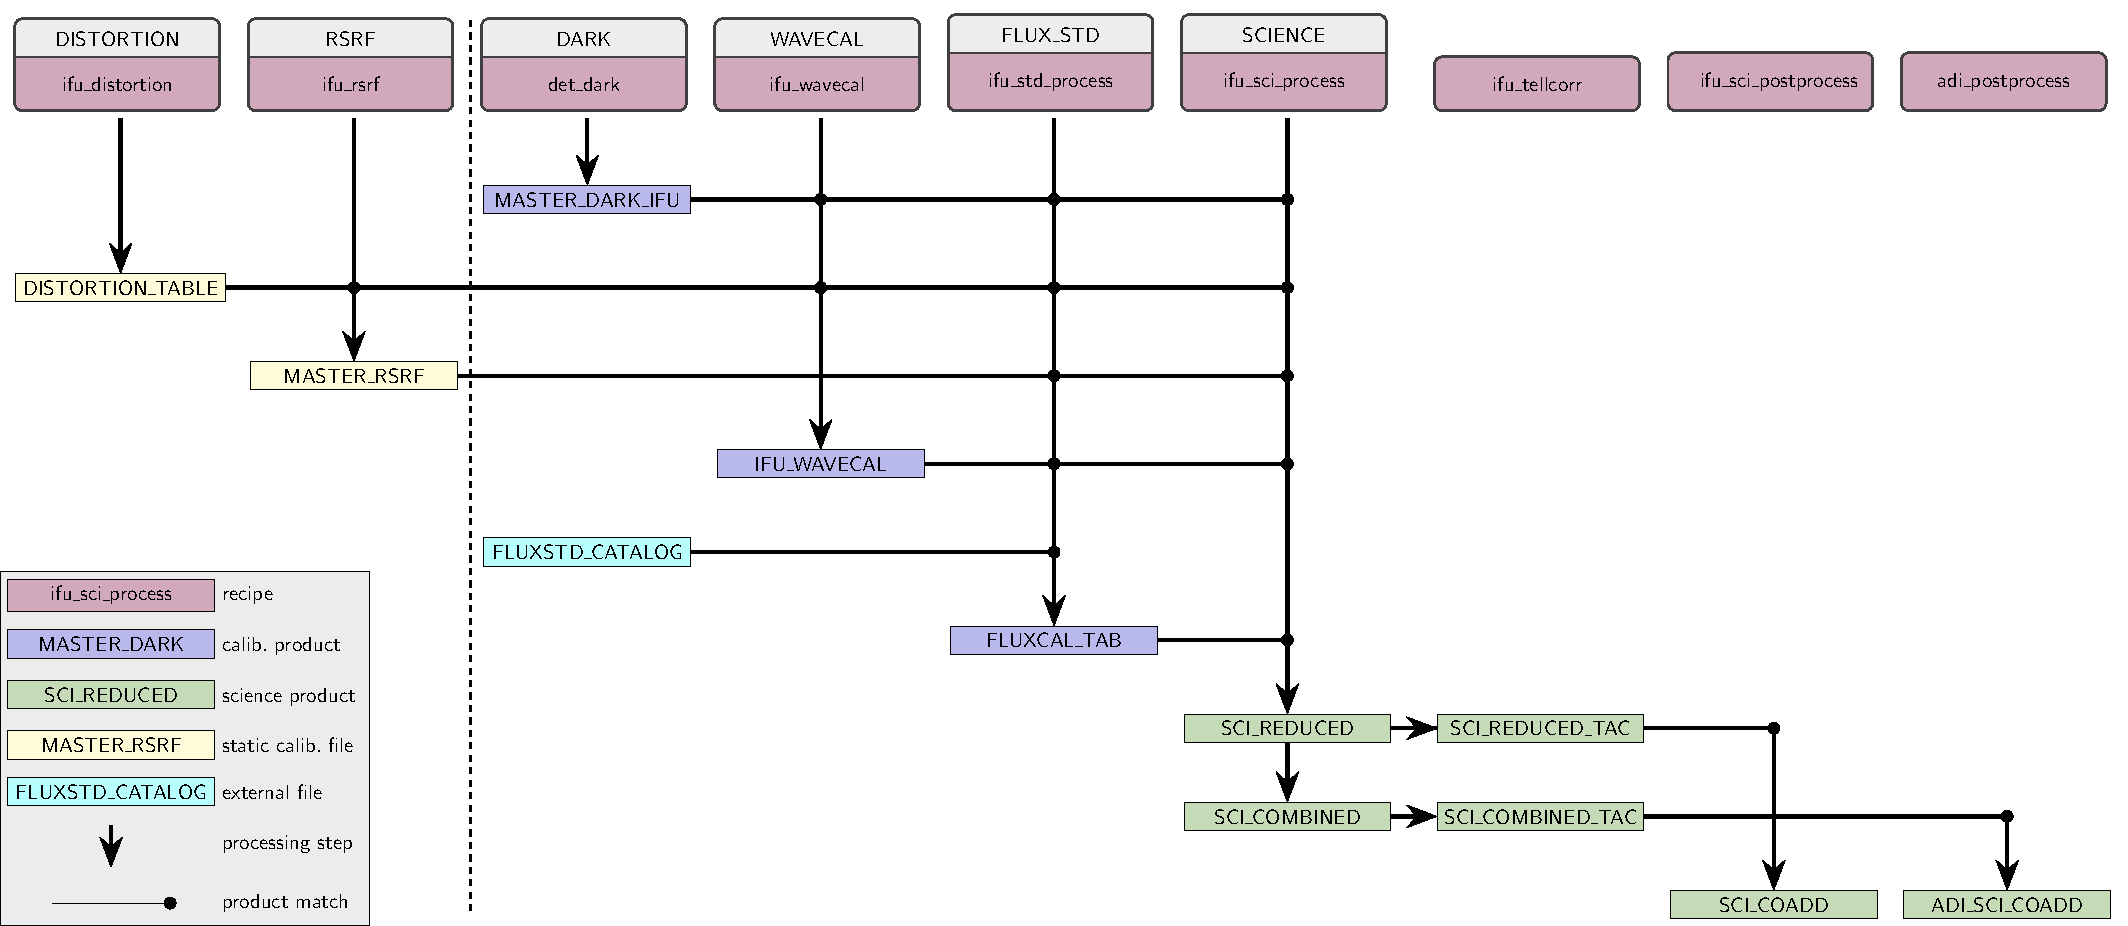
\includegraphics[width=\textheight]{IFU_assomap_tikz}
  \caption[Reduction cascade and association map for IFU
  spectroscopy]{%
    Association map for \ac{IFU} spectroscopy in L- and M-band. The
    figure shows only the primary products created by each recipe; for
    a full list of products refer to the recipe descriptions in
    Sect.~\ref{ssec:IFU_recipes}. The dashed line separates
    calibration tasks that are done at AIT or infrequently during
    operations from tasks done daily. The prefix ``\REC{metis_}'' has been
    omitted from the recipe names to improve clarity.}
  \label{Fig:IfuAssomap}
\end{sidewaysfigure}



%%%%%%%%%%%%%%%%%%%%%%%%%%%%%%%%%%%%%%%%%%%%%%%%%%%%%%

%%% Local Variables:
%%% TeX-master: "METIS_DRLD"
%%% End:


\subsection{Parallel Observing Modes}
\label{ssec:combinedmodes}

There are three parallel observing modes:

\begin{itemize}
\item Parallel observing mode IMG-LM and IMG-N (Section~\ref{sssec:parallellmnimg})
\item Parallel observing mode LSS-LM and LSS-N (Section~\ref{sssec:parallellmnspec})
\item Parallel observing mode IMG-LM and IFU (Section~\ref{sssec:parallellmnspec})
\end{itemize}

The respective templates corresponding to these modes will produce raw data files that can be processed independently by the relevant workflows.
That is, the templates will trigger two different recipe cascades, and there are no specific recipes for any of the parallel observing modes.

\subsubsection{Parallel observing mode IMG-LM and IMG-N}\label{sssec:parallellmnimg}
There are two specific templates for parallel imaging observations in the LM-band and N-band:
\begin{itemize}
 \item \TPL{METIS_img_lmn_obs_AutoChopNod}
 \item \TPL{METIS_img_lmn_obs_GenericChopNod}
\end{itemize}
These templates produce two kind of raw images that are processed independently in either the LM-band or N-band imaging workflow.
This fulfills \REQ{METIS-7244}.


\subsubsection{Parallel observing mode LSS-LM and LSS-N}\label{sssec:parallellmnspec}
There is one specific template for parallel LSS observations in the LM-band and N-band:
\begin{itemize}
 \item \TPL{METIS_spec_lmn_obs_AutoChopNodOnSlit}
\end{itemize}
These templates produce two kind of raw images that are processed independently in either the LM-band or N-band LSS workflow.
This fulfills \REQ{METIS-7245}.

\subsubsection{Parallel observing mode IMG-LM and IFU}\label{sssec:parallellmifu}
Parallel observing mode IMG-LM and IFU is also needed to perform non-common path pointing and aberration correction in \ac{HCI} modes:
real-time monitoring of non-common path aberrations between the \ac{SCAO} \ac{WFS} and the \ac{HCI} elements cannot be performed with the \ac{IFU} due to slicing and sampling issues.

The IFU pickoff optic is a beamsplitter with a transmission of ~10\% to the LM imager and a reflectivity of ~90\% to the IFU. % https://polarion.astron.nl/polarion/#/project/METIS/workitem?id=METIS-3111
LM-band images can therefore be taken in parallel with the IFU exposures, for any of the IFU templates.
The LM-band images and IFU exposures are processed independently.
This fulfills \REQ{METIS-6072}.


\subsection{Workflows}
The association matrices described in the previous sections will be converted one-to-one into Reflex or \ac{EDPS} workflows.

Any interactivity in the workflows is described with the individual recipes.


\subsection{Matched FITS keywords}

The workflow management system (e.g. \ac{EDPS}) uses the `matched keywords'
to find calibration data when processing data.
That is, the system will compare the FITS keywords of the primary input, to
the FITS headers of the pool of possible calibration files to use, in order
to decide what data to use.

For example, most calibration data has to be taken with the same \FITS{DET.DIT}
and \FITS{DET.NDIT} combination as the science data.
Several calibration products also need to use the same filter, or the same mask, or the same grism as the science data.

All selections are done on equality.
That is, no interpolation between, e.g., \FITS{DET.DIT}, will be done if only an approximate matching data product is found.

The following two tables provide an overview of the matched FITS
keywords. Table~\ref{tab:fitskeywordaliasses} defines several high level keyword
aliases used for convenience when there are several combinations
of instrumental keywords (INS.) which are needed to match with the correct
calibration files. These keywords are used in the Matched Keyword
descriptions in the recipes in Chapter~\ref{sec:pipeline_recipes}.
Table~\ref{tab:fitsmatchedkeywordssummary}
summaries the input data, calibration files, and the FITS
keyworlds needed to match them for all the recipes listed in
Chapter~\ref{sec:pipeline_recipes}. The second defines various high
level aliases used for convenience when there are several combinations
of instrumental keywords which are needed to match with the correct
calibration files.

\begin{table}
    \caption{FITS keyword aliases}
    \label{tab:fitskeywordaliasses}
  \begin{tabular}[c]{|p{3cm}|p{5cm}|p{5cm}|}
      \hline
      \textbf{Alias} & \textbf{Description} & \textbf{FITS keywords} \\
      \hline
\FITS{DRS.FILTER}   & Filter Information (LM or N)  & value of \FITS{INS.OPTI10.NAME} or \FITS{INS.OPTI13.NAME} \\
\FITS{DRS.NDFILTER} & ND Filter information	        & value of \FITS{INS.OPTI11.NAME} or \FITS{INS.OPTI13.NAME} \\
\FITS{DRS.SLIT}     & Slit Information (LM or N)    & value of \FITS{INS.OPTI3.NAME} and \FITS{INS.OPTI12.NAME} or  \FITS{INS.OPTI9.NAME} \\
\FITS{DRS.MASK}     & Mask information for Coronagraphy	& value of \FITS{INS.OPTI1.NAME}, \FITS{INS.OPTI3.NAME}, \FITS{INS.OPTI5.NAME}, \FITS{INS.OPTI9.NAME}, \FITS{INS.OPTI12.NAME} \\
\FITS{DRS.PUPIL}    & Pupil information             & value of \FITS{INS.OPTI15.NAME} or \FITS{INS.OPTI16.NAME}\\
\hline
    \end{tabular}
\end{table}


\newgeometry{bottom=0.1cm, right=0.1cm, left=0.1cm, top=0.1cm}
\begin{landscape}
{
  \begin{longtable}[c]{|p{4.2cm}|p{4.6cm}|p{5.6cm}|p{3.5cm}|p{3.5cm}|}
%  \begin{longtable}[c]{|l|l|l|l|l|}
 \caption{FITS matched keywords summary}
 \label{tab:fitsmatchedkeywordssummary}
 \endfirsthead
 \hline
 \textbf{Recipe} & \textbf{Main Input} & \textbf{Calibration Data} & \textbf{FITS keywords} & \textbf{Aliases} \\
 \hline
    \endhead
 \hline
 \textbf{Recipe} & \textbf{Main Input} & \textbf{Calibration Data} & \textbf{FITS keywords} & \textbf{Aliases} \\
 \hline
\REC{metis_det_lingain} & \RAW{DETLIN_det_RAW}, \RAW{det_WCU_OFF_RAW} &  &  &  \\
\REC{metis_det_dark} & \RAW{DARK_det_RAW} & \PROD{LINEARITY_det}, \PROD{PERSISTENCE_MAP} &  &  \\
\REC{metis_det_persistence} &  &  &  &  \\
\REC{metis_lm_img_flat} & \RAW{LM_FLAT_LAMP_RAW}, \RAW{LM_FLAT_TWILIGHT_RAW} & \PROD{MASTER_DARK_2RG} & \FITS{DET.DIT}, \FITS{DET.NDIT}, \FITS{INS.OPTI10.NAME} & \FITS{DET.DIT}, \FITS{DET.NDIT}, \FITS{DRS.FILTER},  \\
\REC{metis_lm_img_basic_reduce} & \RAW{LM_IMAGE_SCI_RAW} & \PROD{MASTER_DARK_2RG}, \PROD{MASTER_IMG_FLAT_LAMP_LM}, \PROD{MASTER_IMG_FLAT_TWILIGHT_LM} & \FITS{DET.DIT}, \FITS{DET.NDIT}, \FITS{INS.OPTI10.NAME} & \FITS{DET.DIT}, \FITS{DET.NDIT}, \FITS{DRS.FILTER},  \\
\REC{metis_lm_img_background} & \RAW{LM_SCI_BASIC_REDUCED}, \RAW{LM_STD_BASIC_REDUCED} &  & \FITS{INS.OPTI10.NAME} & \FITS{DRS.FILTER},  \\
\REC{metis_lm_img_std_process} & \RAW{LM_STD_BKG_SUBTRACTED} & \PROD{FLUXSTD_CATALOG} & \FITS{INS.OPTI10.NAME} & \FITS{DRS.FILTER},  \\
\REC{metis_lm_img_calibrate} & \RAW{LM_SCI_BKG_SUBTRACTED} & \PROD{FLUXCAL_TAB}, \PROD{LM_DISTORTION_TABLE} & \FITS{INS.OPTI10.NAME} & \FITS{DRS.FILTER},  \\
\REC{metis_lm_img_sci_postprocess} & \RAW{LM_SCI_CALIBRATED} &  & \FITS{INS.OPTI10.NAME} & \FITS{DRS.FILTER},  \\
\REC{metis_lm_img_distortion} & \RAW{LM_DISTORTION_RAW}, \RAW{LM_WCU_OFF_RAW} & \EXTCALIB{PINHOLE_TABLE} & \FITS{INS.OPTI10.NAME} & \FITS{DRS.FILTER},  \\
\REC{metis_n_img_flat} & \RAW{N_FLAT_LAMP_RAW}, \RAW{N_FLAT_TWILIGHT_RAW} & \PROD{MASTER_DARK_GEO} & \FITS{DET.DIT}, \FITS{DET.NDIT}, \FITS{INS.OPTI10.NAME} & \FITS{DET.DIT}, \FITS{DET.NDIT}, \FITS{DRS.FILTER},  \\
\REC{metis_n_img_chopnod} & \RAW{N_IMAGE_SCI_RAW} & \PROD{N_FLAT_LAMP_RAW}, \PROD{N_FLAT_TWILIGHT_RAW} & \FITS{DET.DIT}, \FITS{DET.NDIT}, \FITS{INS.OPTI10.NAME} & \FITS{DET.DIT}, \FITS{DET.NDIT}, \FITS{DRS.FILTER},  \\
\REC{metis_n_img_std_process} & \RAW{N_STD_BKG_SUBTRACTED} & \PROD{FLUXSTD_CATALOG} & \FITS{INS.OPTI13.NAME} & \FITS{DRS.FILTER},  \\
\REC{metis_n_img_calibrate} & \RAW{N_SCI_BKG_SUBTRACTED} & \PROD{FLUXCAL_TAB}, \PROD{N_DISTORTION_TABLE} & \FITS{INS.OPTI13.NAME} & \FITS{DRS.FILTER},  \\
\REC{metis_n_img_restore} & \RAW{N_SCI_CALIBRATED} &  & \FITS{INS.OPTI13.NAME} & \FITS{DRS.FILTER},  \\
\REC{metis_n_img_distortion} & \RAW{N_DISTORTION_RAW}, \RAW{N_WCU_OFF_RAW} & \EXTCALIB{PINHOLE_TABLE} & \FITS{INS.OPTI13.NAME} & \FITS{DRS.FILTER},  \\
\REC{metis_LM_lss_rsrf} & \RAW{LM_LSS_RSRF_RAW}, \RAW{LM_WCU_OFF_RAW} & \PROD{LINEARITY_2RG}, \PROD{PERSISTENCE_MAP}, \PROD{GAIN_MAP_2RG}, \PROD{MASTER_DARK_2RG} & \FITS{DET.DIT}, \FITS{DET.NDIT}, \FITS{INS.OPTI9.NAME} & \FITS{DET.DIT}, \FITS{DET.NDIT}, \FITS{DRS.SLIT},  \\
\REC{metis_LM_lss_trace} & \RAW{LM_LSS_RSRF_PINH_RAW}, \RAW{LM_WCU_OFF_RAW} & \PROD{LINEARITY_2RG}, \PROD{PERSISTENCE_MAP}, \PROD{GAIN_MAP_2RG}, \PROD{MASTER_DARK_2RG}, \PROD{MASTER_LM_LSS_RSRF} & \FITS{DET.DIT}, \FITS{DET.NDIT}, \FITS{INS.OPTI9.NAME} & \FITS{DET.DIT}, \FITS{DET.NDIT}, \FITS{DRS.SLIT},  \\
\REC{metis_LM_lss_wave} & \RAW{LM_LSS_WAVE_RAW} & \PROD{LINEARITY_2RG}, \PROD{PERSISTENCE_MAP}, \PROD{GAIN_MAP_2RG}, \PROD{MASTER_DARK_2RG}, \PROD{MASTER_LM_LSS_RSRF}, \PROD{LM_LSS_TRACE}, \PROD{LASER_TAB} & \FITS{DET.DIT}, \FITS{DET.NDIT}, \FITS{INS.OPTI9.NAME}, \FITS{SEQ.WCU.LASERn} & \FITS{DET.DIT}, \FITS{DET.NDIT}, \FITS{DRS.SLIT}, \FITS{SEQ.WCU.LASERn},  \\
\REC{metis_LM_lss_std} & \RAW{LM_LSS_STD_RAW} & \PROD{LINEARITY_2RG}, \PROD{PERSISTENCE_MAP}, \PROD{GAIN_MAP_2RG}, \PROD{MASTER_DARK_2RG}, \PROD{MASTER_LM_LSS_RSRF}, \PROD{LM_LSS_DIST_SOL}, \PROD{LM_LSS_WAVE_GUESS}, \PROD{AO_PSF_MODEL}, \PROD{ATM_LINE_CAT}, \PROD{LM_ADC_SLITLOSS}, \PROD{LM_SYNTH_TRANS}, \PROD{REF_STD_CAT} & \FITS{DET.DIT}, \FITS{DET.NDIT}, \FITS{INS.OPTI9.NAME} & \FITS{DET.DIT}, \FITS{DET.NDIT}, \FITS{DRS.SLIT},  \\
\REC{metis_LM_lss_sci} & \RAW{LM_LSS_SCI_RAW} & \PROD{LINEARITY_2RG}, \PROD{PERSISTENCE_MAP}, \PROD{GAIN_MAP_2RG}, \PROD{MASTER_DARK_2RG}, \PROD{MASTER_LM_LSS_RSRF}, \PROD{LM_LSS_DIST_SOL}, \PROD{LM_LSS_WAVE_GUESS}, \PROD{AO_PSF_MODEL}, \PROD{ATM_LINE_CAT}, \PROD{LM_ADC_SLITLOSS}, \PROD{STD_TRANSMISSION}, \PROD{MASTER_LM_RESPONSE} & \FITS{DET.DIT}, \FITS{DET.NDIT}, \FITS{INS.OPTI9.NAME} & \FITS{DET.DIT}, \FITS{DET.NDIT}, \FITS{DRS.SLIT},  \\
\REC{metis_LM_lss_mf_model} & \RAW{LM_LSS_SCI_FLUX_1D} & \PROD{LSF_KERNEL}, \PROD{ATM_PROFILE}, \PROD{ATM_LINE_CAT} & \FITS{INS.OPTI9.NAME} & \FITS{DRS.SLIT},  \\
\REC{metis_LM_lss_mf_calctrans} & \RAW{MF_BEST_FIT_TAB} & \PROD{LSF_KERNEL}, \PROD{ATM_PROFILE}, \PROD{ATM_LINE_CAT} & \FITS{INS.OPTI9.NAME} & \FITS{DRS.SLIT},  \\
\REC{metis_LM_lss_mf_correct} & \RAW{LM_LSS_SCI_FLUX_1D}, \RAW{LM_LSS_SYNTH_TRANS} &  & \FITS{INS.OPTI9.NAME} & \FITS{DRS.SLIT},  \\
\REC{metis_N_lss_rsrf} & \RAW{N_LSS_RSRF_RAW}, \RAW{N_WCU_OFF_RAW} & \PROD{LINEARITY_GEO}, \PROD{PERSISTENCE_MAP}, \PROD{GAIN_MAP_GEO}, \PROD{MASTER_DARK_GEO} & \FITS{DET.DIT}, \FITS{DET.NDIT}, \FITS{INS.OPTI12.NAME} & \FITS{DET.DIT}, \FITS{DET.NDIT}, \FITS{DRS.SLIT},  \\
\REC{metis_N_lss_trace} & \RAW{N_LSS_RSRF_PINH_RAW}, \RAW{N_WCU_OFF_RAW} & \PROD{LINEARITY_GEO}, \PROD{PERSISTENCE_MAP}, \PROD{GAIN_MAP_GEO}, \PROD{MASTER_DARK_GEO}, \PROD{MASTER_N_LSS_RSRF} & \FITS{DET.DIT}, \FITS{DET.NDIT}, \FITS{INS.OPTI12.NAME} & \FITS{DET.DIT}, \FITS{DET.NDIT}, \FITS{DRS.SLIT},  \\
%\REC{metis_N_lss_wave} & \RAW{N_LSS_WAVE_RAW} & \PROD{LINEARITY_GEO}, \PROD{PERSISTENCE_MAP}, \PROD{GAIN_MAP_GEO}, \PROD{MASTER_DARK_GEO}, \PROD{MASTER_N_LSS_RSRF}, \PROD{N_LSS_TRACE}, \PROD{LASER_TAB} & \FITS{DET.DIT}, \FITS{DET.NDIT}, \FITS{INS.OPTI12.NAME}, \FITS{SEQ.WCU.LASERn} & \FITS{DET.DIT}, \FITS{DET.NDIT}, \FITS{DRS.SLIT}, \FITS{SEQ.WCU.LASERn},  \\
\REC{metis_N_lss_std} & \RAW{N_LSS_STD_RAW} & \PROD{LINEARITY_GEO}, \PROD{PERSISTENCE_MAP}, \PROD{GAIN_MAP_GEO}, \PROD{MASTER_DARK_GEO}, \PROD{MASTER_N_LSS_RSRF}, \PROD{N_LSS_DIST_SOL}, \PROD{N_LSS_WAVE_GUESS}, \PROD{AO_PSF_MODEL}, \PROD{ATM_LINE_CAT}, \PROD{N_ADC_SLITLOSS}, \PROD{N_SYNTH_TRANS}, \PROD{REF_STD_CAT} & \FITS{DET.DIT}, \FITS{DET.NDIT}, \FITS{INS.OPTI12.NAME} & \FITS{DET.DIT}, \FITS{DET.NDIT}, \FITS{DRS.SLIT},  \\
\REC{metis_N_lss_sci} & \RAW{N_LSS_SCI_RAW} & \PROD{LINEARITY_GEO}, \PROD{PERSISTENCE_MAP}, \PROD{GAIN_MAP_GEO}, \PROD{MASTER_DARK_GEO}, \PROD{MASTER_N_LSS_RSRF}, \PROD{N_LSS_DIST_SOL}, \PROD{N_LSS_WAVE_GUESS}, \PROD{AO_PSF_MODEL}, \PROD{ATM_LINE_CAT}, \PROD{N_ADC_SLITLOSS}, \PROD{STD_TRANSMISSION}, \PROD{MASTER_N_RESPONSE} & \FITS{DET.DIT}, \FITS{DET.NDIT}, \FITS{INS.OPTI12.NAME} & \FITS{DET.DIT}, \FITS{DET.NDIT}, \FITS{DRS.SLIT},  \\
\REC{metis_N_lss_mf_model} & \RAW{N_LSS_SCI_FLUX_1D} & \PROD{LSF_KERNEL}, \PROD{ATM_PROFILE}, \PROD{ATM_LINE_CAT} & \FITS{INS.OPTI12.NAME} & \FITS{DRS.SLIT},  \\
\REC{metis_N_lss_mf_calctrans} & \RAW{MF_BEST_FIT_TAB} & \PROD{LSF_KERNEL}, \PROD{ATM_PROFILE}, \PROD{ATM_LINE_CAT} & \FITS{INS.OPTI12.NAME} & \FITS{DRS.SLIT},  \\
\REC{metis_N_lss_mf_correct} & \RAW{N_LSS_SCI_FLUX_1D}, \RAW{N_LSS_SYNTH_TRANS} &  & \FITS{INS.OPTI12.NAME} & \FITS{DRS.SLIT},  \\
\REC{metis_ifu_wavecal} & \RAW{IFU_WAVE_RAW} & \PROD{MASTER_DARK_IFU}, \PROD{IFU_DISTORTION_TABLE} & \FITS{DET.DIT}, \FITS{DET.NDIT}, \FITS{INS.OPTI6.NAME} & \FITS{DET.DIT}, \FITS{DET.NDIT}, \FITS{DRS.IFU},  \\
\REC{metis_ifu_rsrf} & \RAW{IFU_RSRF_RAW} & \PROD{MASTER_DARK_IFU}, \PROD{IFU_WAVECAL} & \FITS{DET.DIT}, \FITS{DET.NDIT}, \FITS{INS.OPTI6.NAME} & \FITS{DET.DIT}, \FITS{DET.NDIT}, \FITS{DRS.IFU},  \\
\REC{metis_ifu_calibrate} & \RAW{IFU_STD_RAW} & \PROD{MASTER_DARK_IFU}, \PROD{RSRF_IFU}, \PROD{IFU_WAVECAL}, \PROD{IFU_DISTORTION_TABLE} & \FITS{DET.DIT}, \FITS{DET.NDIT}, \FITS{INS.OPTI6.NAME} & \FITS{DET.DIT}, \FITS{DET.NDIT}, \FITS{DRS.IFU},  \\
\REC{metis_ifu_telluric} & \RAW{IFU_SCI_COMBINED} & \PROD{LSF_KERNEL}, \PROD{ATM_PROFILE} & \FITS{DET.DIT}, \FITS{DET.NDIT}, \FITS{INS.OPTI6.NAME} & \FITS{DET.DIT}, \FITS{DET.NDIT}, \FITS{DRS.IFU},  \\
\REC{metis_ifu_calibrate} & \RAW{IFU_SCI_REDUCED}, \PROD{FLUXCAL_TAB} &  & \FITS{INS.OPTI6.NAME} & \FITS{DRS.IFU},  \\
\REC{metis_ifu_postprocess} & \RAW{IFU_SCI_REDUCED} &  & \FITS{INS.OPTI6.NAME} & \FITS{DRS.IFU},  \\
\REC{metis_ifu_distortion} & \RAW{IFU_DISTORTION_RAW} & \EXTCALIB{PINHOLE_TABLE} & \FITS{INS.OPTI6.NAME} & \FITS{DRS.IFU},  \\
\REC{metis_img_adi_cgrph} & \RAW{LM_SCI_BASIC_REDUCED}, \RAW{N_SCI_BKG_SUBTRACTED} & \PROD{LM_DISTORTION_TABLE}, \PROD{N_DISTORTION_TABLE}, \PROD{LM_cgrph_SCI_THROUGHPUT}, \PROD{N_cgrph_SCI_THROUGHPUT} & \FITS{INS.OPTI1.NAME}, \FITS{INS.OPTI3.NAME}, \FITS{INS.OPTI5.NAME}, \FITS{INS.OPTI9.NAME}, \FITS{INS.OPTI10.NAME}, \FITS{INS.OPTI13.NAME} & \FITS{DRS.MASK},  \\
\REC{metis_lm_adi_app} & \RAW{LM_SCI_BASIC_REDUCED} & \PROD{LM_DISTORTION_TABLE}, \PROD{LM_OFF_AXIS_PSF_RAW} & \FITS{INS.OPTI5.NAME}, \FITS{INS.OPTI9.NAME}, \FITS{INS.OPTI10.NAME} & \FITS{DRS.MASK},  \\
\REC{metis_ifu_adi_cgrph} & \RAW{IFU_SCI_REDUCED} & \PROD{IFU_DISTORTION_TABLE}, \PROD{IFU_cgrph_SCI_THROUGHPUT} & \FITS{INS.OPTI6.NAME}, \FITS{INS.OPTI1.NAME}, \FITS{INS.OPTI3.NAME}, \FITS{INS.OPTI5.NAME}, \FITS{INS.OPTI9.NAME}, \FITS{INS.OPTI12.NAME} & \FITS{DRS.MASK},  \\
\REC{metis_pupil_imaging} & \RAW{LM_PUPIL_RAW}, \RAW{N_PUPIL_RAW} &  & \FITS{INS.OPTI15.NAME}, \FITS{INS.OPTI16.NAME}, \FITS{INS.OPTI10.NAME}, \FITS{INS.OPTI13.NAME} & \FITS{DRS.PUPIL},  \\
\REC{metis_cal_chophome} & \RAW{LM_CHOPHOME_RAW} & \PROD{LINEARITY_2RG}, \PROD{PERSISTENCE_MAP}, \PROD{GAIN_MAP_2RG}, \PROD{MASTER_DARK_2RG}, \PROD{MASTER_IMG_FLAT_LAMP_LM} & \FITS{DET.DIT}, \FITS{DET.NDIT}, \FITS{INS.OPTI10.NAME} & \FITS{DET.DIT}, \FITS{DET.NDIT}, \FITS{DRS.FILTER},  \\
\REC{metis_lm_adc_slitloss} & \RAW{LM_SLITLOSSES_RAW}, \RAW{LM_WCU_OFF_RAW} & \PROD{LINEARITY_2RG}, \PROD{PERSISTENCE_MAP}, \PROD{GAIN_MAP_2RG}, \PROD{MASTER_DARK_2RG}, \PROD{MASTER_IMG_FLAT_LAMP_LM} & \FITS{INS.OPTI10.NAME}, \FITS{INS.OPTI13.NAME} & \FITS{DET.DIT}, \FITS{DET.NDIT}, \FITS{DRS.FILTER},  \\
\REC{metis_n_adc_slitloss} & \RAW{LM_SLITLOSSES_RAW}, \RAW{LM_WCU_OFF_RAW} & \PROD{LINEARITY_GEO}, \PROD{PERSISTENCE_MAP}, \PROD{GAIN_MAP_GEO}, \PROD{MASTER_DARK_GEO}, \PROD{MASTER_IMG_FLAT_LAMP_N} & \FITS{INS.OPTI10.NAME}, \FITS{INS.OPTI13.NAME} & \FITS{DET.DIT}, \FITS{DET.NDIT}, \FITS{DRS.FILTER},  \\
    \hline
    \end{longtable}
  }
\end{landscape}
\restoregeometry

%%% Local Variables:
%%% TeX-master: "METIS_DRLD"
%%% End:
